\documentclass[runningheads]{llncs}
\usepackage[ruled]{algorithm2e}
\usepackage{amsfonts}
\usepackage{amsmath}
\usepackage{bm}
\usepackage{booktabs}
\usepackage{color}
\usepackage[compress]{cite}
\usepackage{graphicx}
\usepackage{hyperref}
\usepackage{physics}

\renewcommand\UrlFont{\color{blue}\rmfamily}
\SetKwInput{KwHyperparameters}{Hyperparameters}
\DeclareMathOperator{\sgn}{sgn}
\DeclareMathOperator*{\argmax}{arg\,max}

\begin{document}

\title{
    Multiclass Classification with Pegasos
}
\author{Gabriele Cerizza}
\authorrunning{G. Cerizza}

\institute{Università degli Studi di Milano\\
\email{gabriele.cerizza@studenti.unimi.it}\\
\url{https://github.com/gabrielecerizza/smml}}

\maketitle

\section*{Introduction}
\label{sec:introduction}

In this report we detail the results of our experiments on the Pegasos algorithm~\cite{shalev-pegasos-2011} over a multiclass classification task, pursuant to the project specifications set out for the Statistical Methods for Machine Learning course of the Università degli Studi di Milano\footnote{\url{https://cesa-bianchi.di.unimi.it/MSA/index\_21-22.html}}. 

In Section~\ref{sec:dataset} we illustrate the dataset used in the experiments. In Section~\ref{sec:algorithm} we briefly describe the algorithm and its implementation. In Section~\ref{sec:experiments} we show the results of our experiments and provide comments on them. Finally, Section~\ref{sec:conclusions} contains our concluding remarks. 

\section{Dataset}
\label{sec:dataset}

Our analysis was carried out on the USPS dataset\footnote{\url{https://www.kaggle.com/datasets/bistaumanga/usps-dataset}}, comprising 9298 $16\times16$ grayscale images. These images depict handwritten digits ranging from 0 to 9. A sample of these digits can be seen in Figure~\ref{fig:dataset:digits}. The classes do not present severe imbalance issues, as shown in Figure~\ref{fig:dataset:class_counts}. The values of the examples are scaled in the interval $[0, 1]$.

To gauge the complexity of multiclass classification on this dataset, we performed dimensionality reduction by way of  t-distributed Stochastic Neighbor Embedding (t-SNE)~\cite{maaten-2008-tsne} and projected the examples onto a two-dimensional space. The result is given in Figure~\ref{fig:dataset:tsne}. Within this figure the examples are clustered into ten clearly distinguishable groups, thus suggesting a low complexity classification task.   

The USPS dataset is made available with predetermined training and test sets. In our experiments, however, we merged these sets and run a 5-fold cross-validation on the whole dataset, as illustrated in Section~\ref{sec:experiments}. 

\begin{figure}
  \center
  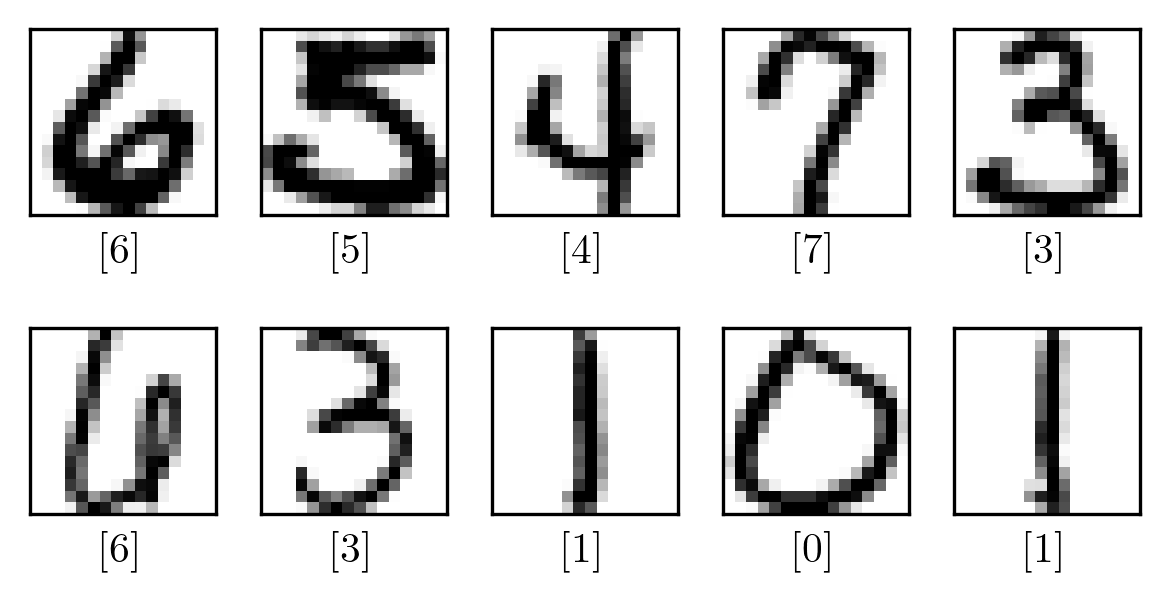
\includegraphics[width=0.7\textwidth]{../img/digits.png}
  \caption{Sample of images from the USPS dataset. The label is indicated below each image.} 
  \label{fig:dataset:digits}
\end{figure}

\begin{figure}
  \center
  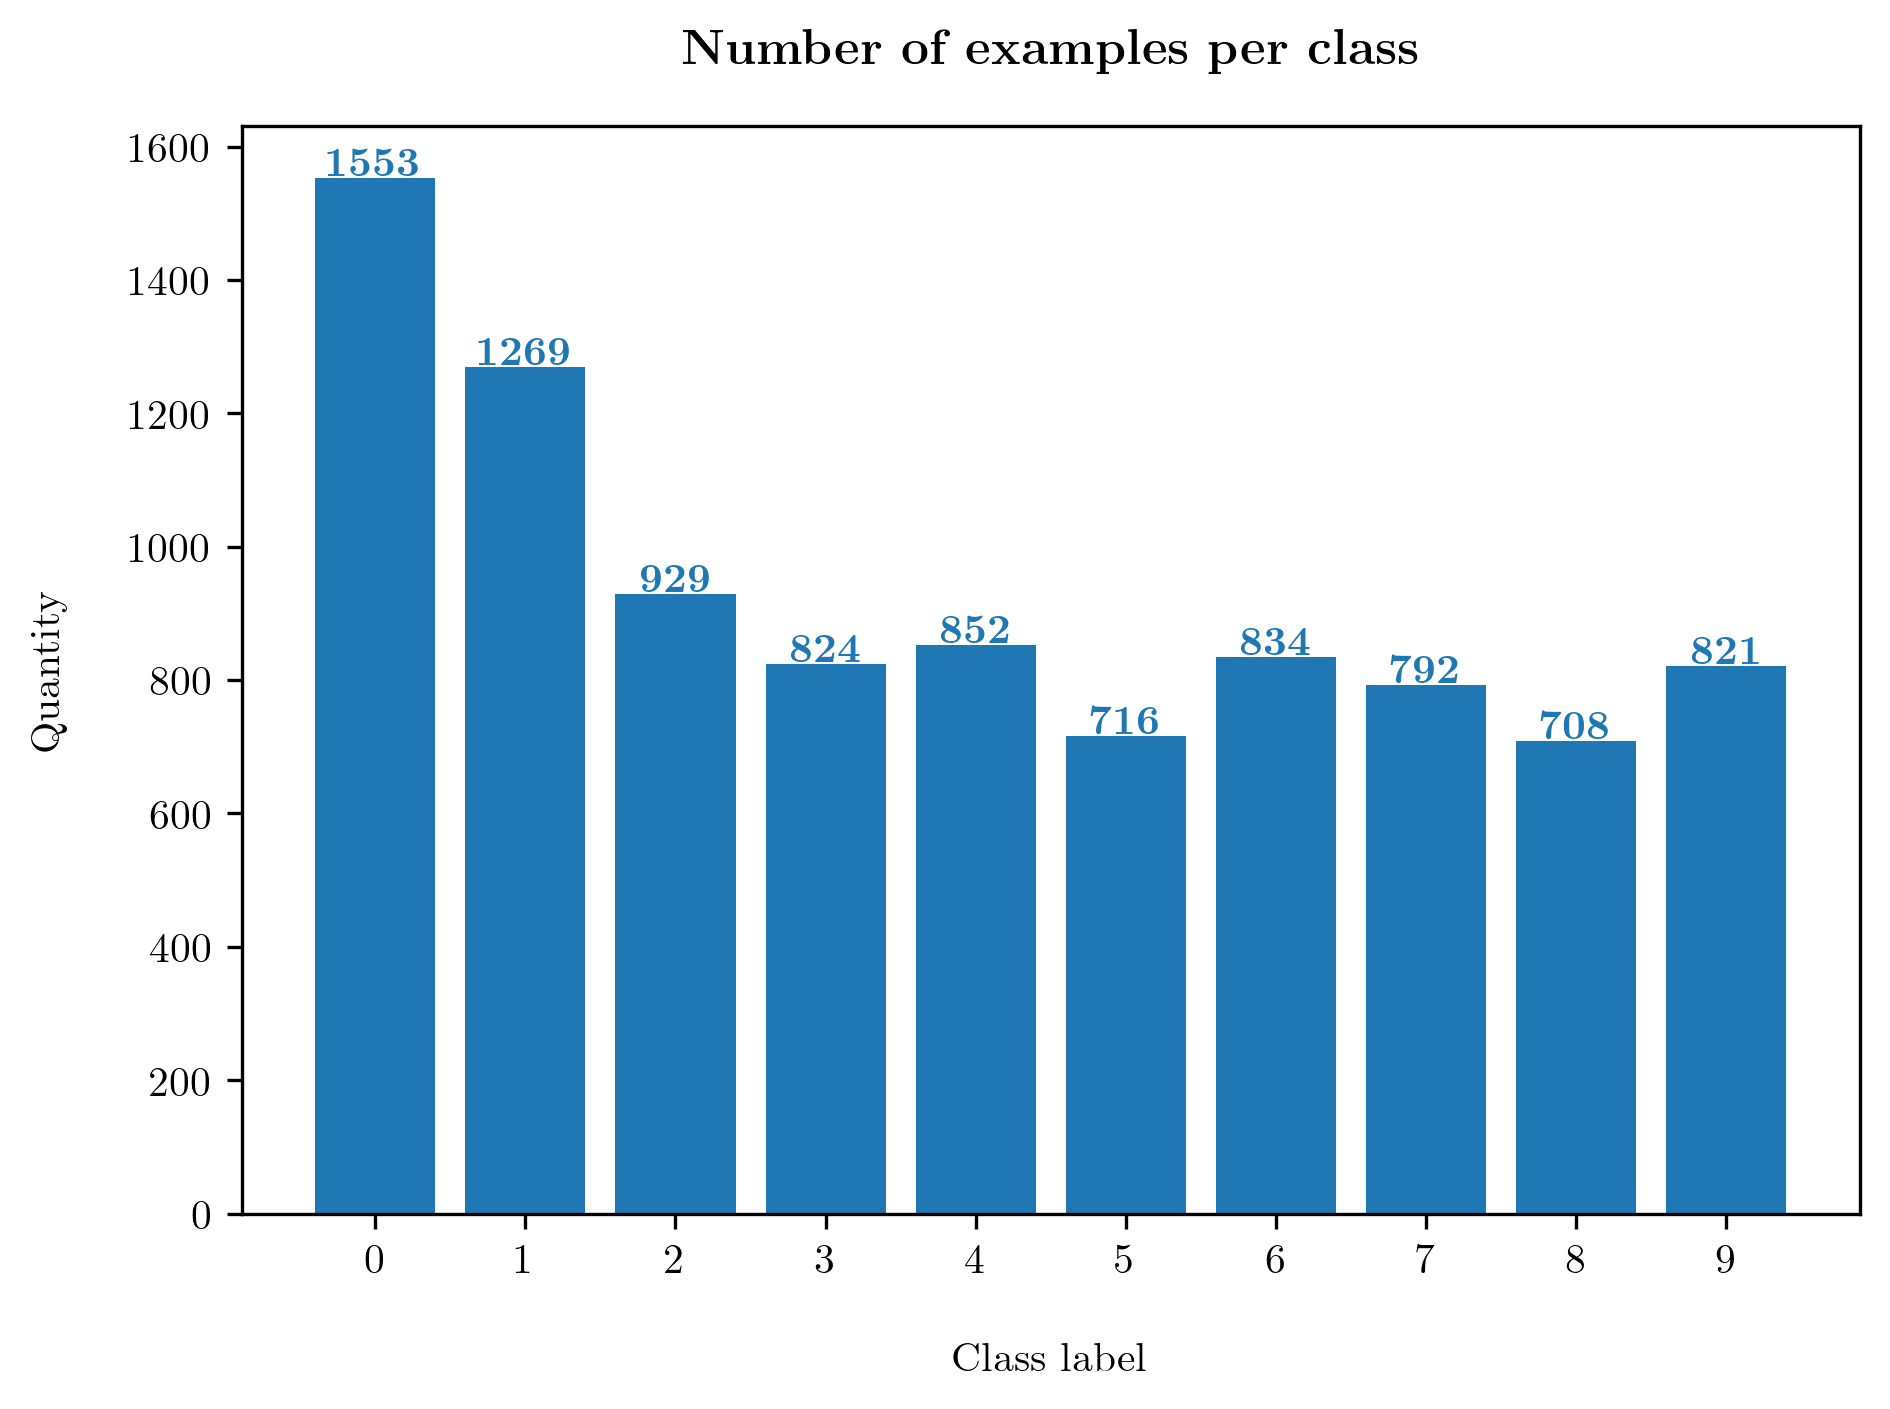
\includegraphics[width=1\textwidth]{../img/class_counts.png}
  \caption{Frequency of the classes in the USPS dataset.} 
  \label{fig:dataset:class_counts}
\end{figure}

\begin{figure}
  \center
  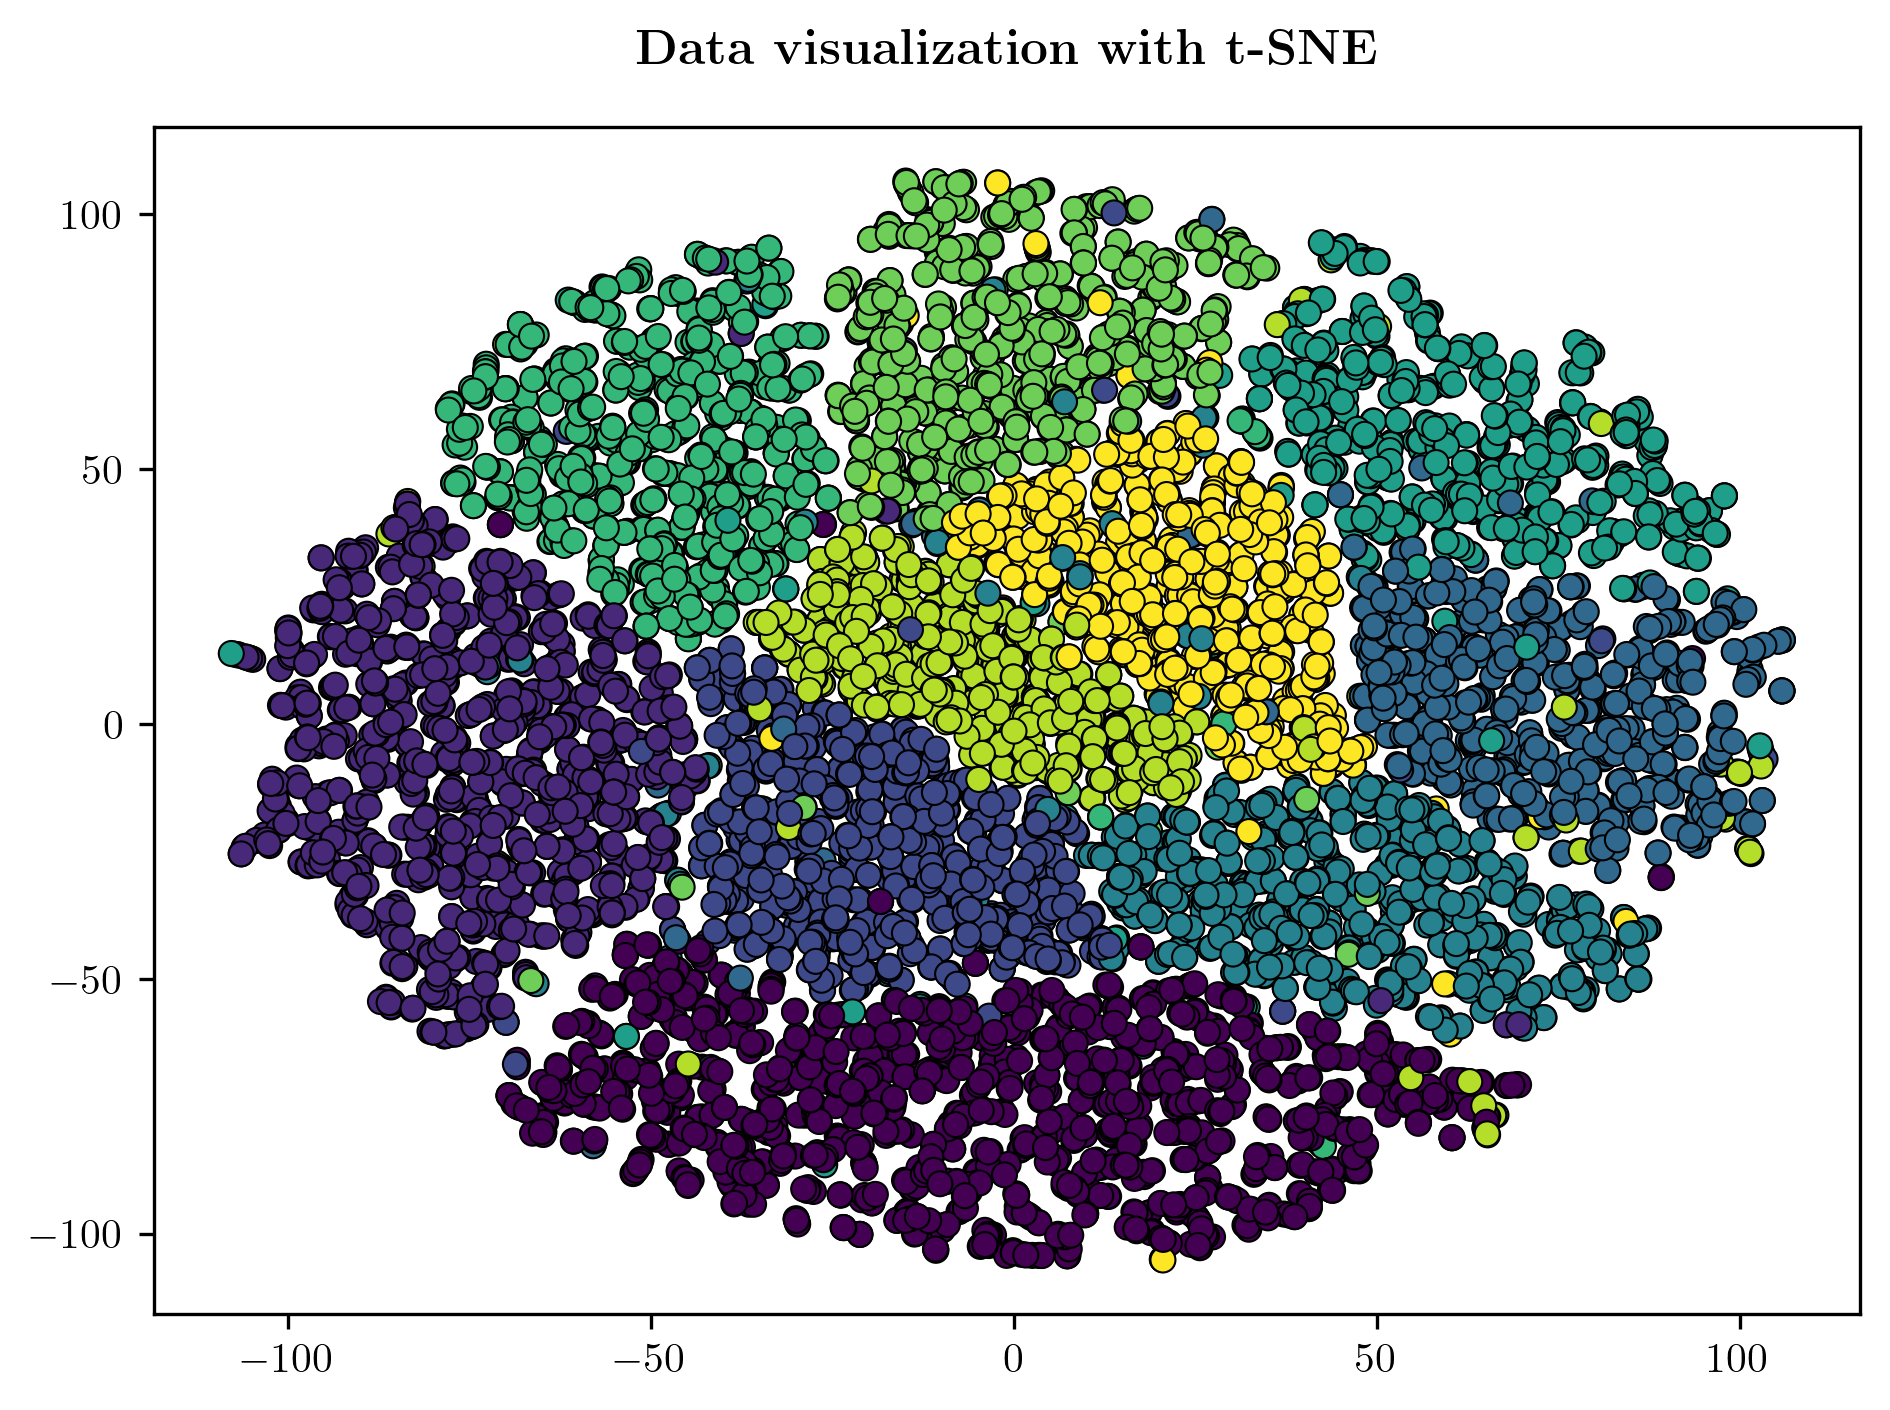
\includegraphics[width=0.9\textwidth]{../img/tsne.png}
  \caption{Projection of the USPS dataset onto a two-dimensional space using t-SNE.} 
  \label{fig:dataset:tsne}
\end{figure}

\section{Pegasos Algorithm}
\label{sec:algorithm}

In the present section we describe the Pegasos algorithm (Section~\ref{subsec:algorithm:description}), the kernel functions employed in our experiments (Section~\ref{subsec:algorithm:kernel}), and some implementation details to reduce the runtime of the algorithm (Section~\ref{subsec:algorithm:implementation}).

\subsection{Description}
\label{subsec:algorithm:description}

The Pegasos algorithm~\cite{shalev-pegasos-2011} was introduced to solve the Support Vector Machine (SVM)~\cite{vapnik-1999-statistical-learning} convex optimization problem for binary classification, which can be formalized as follows. 

Let $S = \{(\bm{x}_1,y_1),\dots,(\bm{x}_m,y_m)\}$ be a training set with $\bm{x}_t \in \mathbb{R}^d, \, y_t \in \{-1, 1\}$ $\forall t=1,\dots,m$; and let $\phi_K : \mathbb{R}^d \to \mathcal{H}_K$ be a function such that $\text{dim}(\mathcal{H}_K) \gg d$ and $\langle \cdot , \cdot \rangle_K$ is the inner product in $\mathcal{H}_K$. The optimization problem aims to find the maximum margin separating hyperplane in $\mathcal{H}_K$, which separates the examples according to their labels and maximizes the distance between the hyperplane and the closest example. This yields the following quadratic programming problem: 
\begin{alignat}{3}
  &\min_{g \in \mathcal{H}_K, \bm{\xi} \in \mathbb{R}^m} & \quad & \frac{\lambda}{2} \norm{g}_K^2 + \frac{1}{m}\sum_{t=1}^{m} \xi_t \, , \notag\\
  &\text{subject to}  &       & y_t \langle g, \phi_K(\bm{x}_t) \rangle_K \geq 1 - \xi_t &\qquad& t = 1,\dots,m \, , \notag\\
  &                   &       & \xi_t \geq 0  &\qquad& t = 1,\dots,m \, , \notag
\end{alignat}
where $\lambda$ is a regularization coefficient dictating the relative importance of the two terms in the objective function; and $\xi_t$ are slack variables that allow, but penalize, examples lying on the wrong side of the hyperplane.

This formulation can be turned into the following unconstrained optimization problem:
\[
  \min_{g \in \mathcal{H}_K} \quad \frac{\lambda}{2} \norm{g}_K^2 + \frac{1}{m}\sum_{t=1}^{m} h_t(g) \, ,
\]
where $h_t(g) = [1 - y_t\langle g, \phi_K(\bm{x}_t) \rangle_K]_+$ is the hinge loss.

Pegasos solves this optimization problem using a stochastic gradient descent approach. The algorithm performs $T$ iterations, each of which consists in drawing a training example uniformly at random and updating $g$ through a gradient step. In particular, at iteration $t$ Pegasos computes
\begin{equation}
  g_{t+1} = \frac{1}{\lambda t} \sum_{r = 1}^{t} \mathbb{I}\{h_{s_r}(g_r) > 0\} y_{s_r} K(\bm{x}_{s_r}, \cdot) \, , \label{eqn:pegasos:g}
\end{equation}
where $\mathbb{I}$ is the indicator function, $s_r$ is the index of the training example randomly drawn at iteration $r$, and $K : \mathbb{R}^d \times \mathbb{R}^d \to \mathbb{R}$ is a kernel function such that $K(\bm{x},\bm{x}^\prime) = \langle \phi_K(\bm{x}), \phi_K(\bm{x}^\prime) \rangle_K$.

Note that $g_{t+1}$ is a function, not a vector. Indeed, the dot in $K(\bm{x}_{s_r}, \cdot)$ stands for a missing argument, corresponding to the example on which the function is evaluated. Therefore, unlike vectors, $g_{t+1}$ cannot be stored in memory and used to perform inference on new examples, since we have to evaluate $g_{t+1}$ on them first.

In order to simplify the process, it was observed in~\cite{shalev-pegasos-2011} that~(\ref{eqn:pegasos:g}) can be rewritten as
\[
  g_{t+1} = \frac{1}{\lambda t} \sum_{j = 1}^{m} \bm{\alpha}_{t+1}[j] y_j K(\bm{x}_j, \cdot) \, ,
\]
where $\bm{\alpha}_{t+1} \in \mathbb{R}^m$ is a vector representing how many times each example $\bm{x}_j$ in the training set has been drawn and resulted in a non-zero loss, that is
\[
  \bm{\alpha}_{t+1}[j] = 	\lvert \{r \leq t : s_r = j \land y_j\langle g_r, \phi_K(\bm{x}_j) \rangle_K < 1 \} \rvert \, .
\]
The vector $\bm{\alpha}_{t+1}$ can be kept in memory and used to quickly evaluate $g_{t+1}$ on new examples during both training and test. Algorithm~\ref{alg:pegasos} shows the pseudocode for the kernelized Pegasos algorithm using the abovementioned approach.    

\begin{algorithm}
  \DontPrintSemicolon
  \caption{Pegasos algorithm in a kernel space}\label{alg:pegasos}
  \KwHyperparameters{$T$, $\lambda > 0$}
  \KwData{Training set $S = \{(\bm{x}_1,y_1),\dots,(\bm{x}_m,y_m)\}$}
  $\bm{\alpha}_1 \gets (0,\dots,0)$\;
  \For{$t=1$ \KwTo $T$}{   
    Choose $s_r \in \{0,\dots, \lvert S \rvert\}$ uniformly at random \;
    \If{$y_{s_r}\frac{1}{\lambda t} \sum_{j = 1}^{m} \bm{\alpha}_{t}[j] y_j K(\bm{x}_j, \bm{x}_{s_r}) < 1$}{
      $\bm{\alpha}_{t+1}[s_r] = \bm{\alpha}_{t}[s_r] + 1$\;
    }
  }
  \Return $\bm{\alpha}_{T+1}$
\end{algorithm}

Once the vector $\bm{\alpha}_{T+1}$ has been obtained, the label of a new example $\bm{x}$ can be predicted by computing
\begin{equation}
  \hat{y} = \sgn \left( \sum_{j = 1}^{m} \bm{\alpha}_{T+1}[j] y_j K(\bm{x}_j, \bm{x}) \right) \, .
\end{equation}
It is not necessary to multiply the sum by $\frac{1}{\lambda T}$, since scaling does not affect the sign.

So far we illustrated the Pegasos algorithm for binary classification. In order to handle multiclass classification, we can adopt the one-vs-all multiclass strategy. We prepare a different binary classifier for each class. These binary classifiers are trained using labels encoded as $1$ for the examples belonging to the class of the classifier, and encoded as $-1$ for the examples belonging to all the other classes. 

Finally, to determine the class of a new example $\bm{x}$, we first compute
\begin{equation}
  h_i = \sum_{j = 1}^{m} \bm{\alpha}_{T+1}[j] y_j K(\bm{x}_j, \bm{x}) \,
  \label{eqn:pegasos:h_i}
\end{equation}
for each classifier $c_i$, and then predict with
\[
  \hat{y} = \argmax_i {h_i} \, .
\]
Also in this case scaling $h_i$ is unnecessary, given that $\frac{1}{\lambda T}$ is always positive and therefore does not change the order of the $h_i$ values.

% What sets the Pegasos algorithm apart from other algorithms developed to solve the SVM problem is its ability to converge to a solution that differs from the optimal solution by less than $\epsilon$ in $O(\frac{1}{\lambda \epsilon})$ iterations with high probability with respect to the random draws of the training examples. In other terms, the convergence rate does not depend on the size of the training set, but only on the number of iterations, making Pegasos a suitable algorithm to perform classification over large datasets.  

\subsection{Kernel functions}
\label{subsec:algorithm:kernel}

In our experiments with the Pegasos algorithm, we employed two kernel functions: the Gaussian kernel and the polynomial kernel. The Gaussian kernel is defined as
\begin{equation}
  K(\bm{x},\bm{x}^\prime) = \exp(-\frac{1}{2 \gamma}\norm{\bm{x} - \bm{x}^\prime}^2) \, , \label{eqn:kernel:gaussian}
\end{equation}
with $\gamma > 0$. The polynomial kernel is defined as
\begin{equation}
  K(\bm{x},\bm{x}^\prime) = (1 + \bm{x}^\top \bm{x}^\prime)^n \, , \label{eqn:kernel:polynomial} 
\end{equation}
where $n \in \mathbb{N}$ is the degree of the polynomial. 

\subsection{Implementation}
\label{subsec:algorithm:implementation}

In this section we expound on two implementation details that improve the runtime of the algorithm.

\subsubsection{Kernel matrix.} In order to perform multiclass classification, we need to train multiple classifiers, each running the Pegasos algorithm over the same training set. Within this framework, the kernel function between two given examples may be computed multiple times, resulting in redundant computations.

Moreover, at each iteration the Pegasos algorithm computes the kernel function between a randomly drawn training example and all the other training examples. Drawing the same example multiple times results in further redundant computations.

Redundant computations adversely affect the runtime of the algorithm and should therefore be avoided. To this effect, we opted to compute ahead of time the kernel matrix $K \in \mathbb{R}^{m \times m}$, such that
\[
  K_{i,j} = K(\bm{x}_i, \bm{x}_j) \quad \forall i,j=1,\dots,m \, .
\]
This matrix was then dispatched to each classifier and used in place of the kernel function evaluation.

The drawback of the kernel matrix lies in its memory footprint. However, given the number of examples in the USPS dataset, such a matrix would require at most $\frac{9298 \times 9298 \times 32}{2^3 \times 10^9} \approx 0.34$ gigabytes of memory, which in modern machines constitutes a negligible amount.  

\subsubsection{Vectorization.} The summations within the Pegasos algorithm can be vectorized, thus allowing to exploit the highly optimized array operations made available by math libraries.

In particular, the condition of the \texttt{if} statement within Algorithm~\ref{alg:pegasos} can be rewritten as
\[
  y_{s_r}\frac{1}{\lambda t} (\bm{\alpha}_t \odot y)^\top K_{s_r} < 1 \, ,
\]
where $\odot$ is the Hadamard product and $K$ is the kernel matrix between the training examples. Likewise, the formula for $h_i$ in (\ref{eqn:pegasos:h_i}) can be rewritten as
\[
  \bm{h}_i = (\bm{\alpha}_{T+1} \odot y)^\top K^\prime \, ,
\]
where $K^\prime$ is the kernel matrix between the test examples and the training examples and $\bm{h}_i$ is the vector containing the predictions for all the test examples returned by classifier $c_i$.

Also the computation of the kernel matrices can be vectorized. In the case of the polynomial kernel, the vectorization is trivial, since the dot product between vectors in~(\ref{eqn:kernel:polynomial}) directly translates into a matrix product. In the case of the Gaussian kernel, however, an analogous approach would fail, because subtracting the training set matrix from itself in~(\ref{eqn:kernel:gaussian}) would result in a null matrix. We therefore followed another approach.

Let $S \in \mathbb{R}^{n \times m}$ be a training set. In order to vectorize the kernel matrix with respect to the Gaussian kernel, we need to compute the difference between each row in $S$ and all the rows in $S$. To accomplish this, we first turn $S$ into a tensor $T \in \mathbb{R}^{n \times 1 \times m}$, in which each row $T_i$ is a $1 \times m$ matrix containing only the corresponding row $S_i$ of the original matrix. Then, we simply compute
\[
  R = T - S \, ,
\]
where $R \in \mathbb{R}^{n \times n \times m}$ is a tensor having $R_i = S_i - S \; \forall i=1,\dots,n$, in which $S_i$ is casted into a $\mathbb{R}^{n \times m}$ matrix using broadcasting rules\footnote{\url{https://numpy.org/doc/stable/user/basics.broadcasting.html}}. Once $R$ is obtained, the Gaussian kernel formula in~\ref{eqn:kernel:gaussian} can be applied straightforwardly. The same procedure can be applied when computing the kernel matrix between the test and training examples.

One caveat of this approach is that $R$ has a much larger memory footprint than the $n \times n$ kernel matrix. At most, the required memory for the USPS dataset would be $0.34 \times 256 \approx 87$ gigabytes. For this reason, it is necessary to split $S$ into chunks, apply the procedure on each chunk and then concatenate the results.

\subsubsection{Comparison.} The training runtime reduction obtained by applying the abovementioned optimizations on a single binary classifier is given in Figure~\ref{fig:algorithm:runtime}. The shown improvement becomes even more prominent when accounting the fact that, for multiclass classification, multiple classifiers need to be trained.

\begin{figure}
  \center
  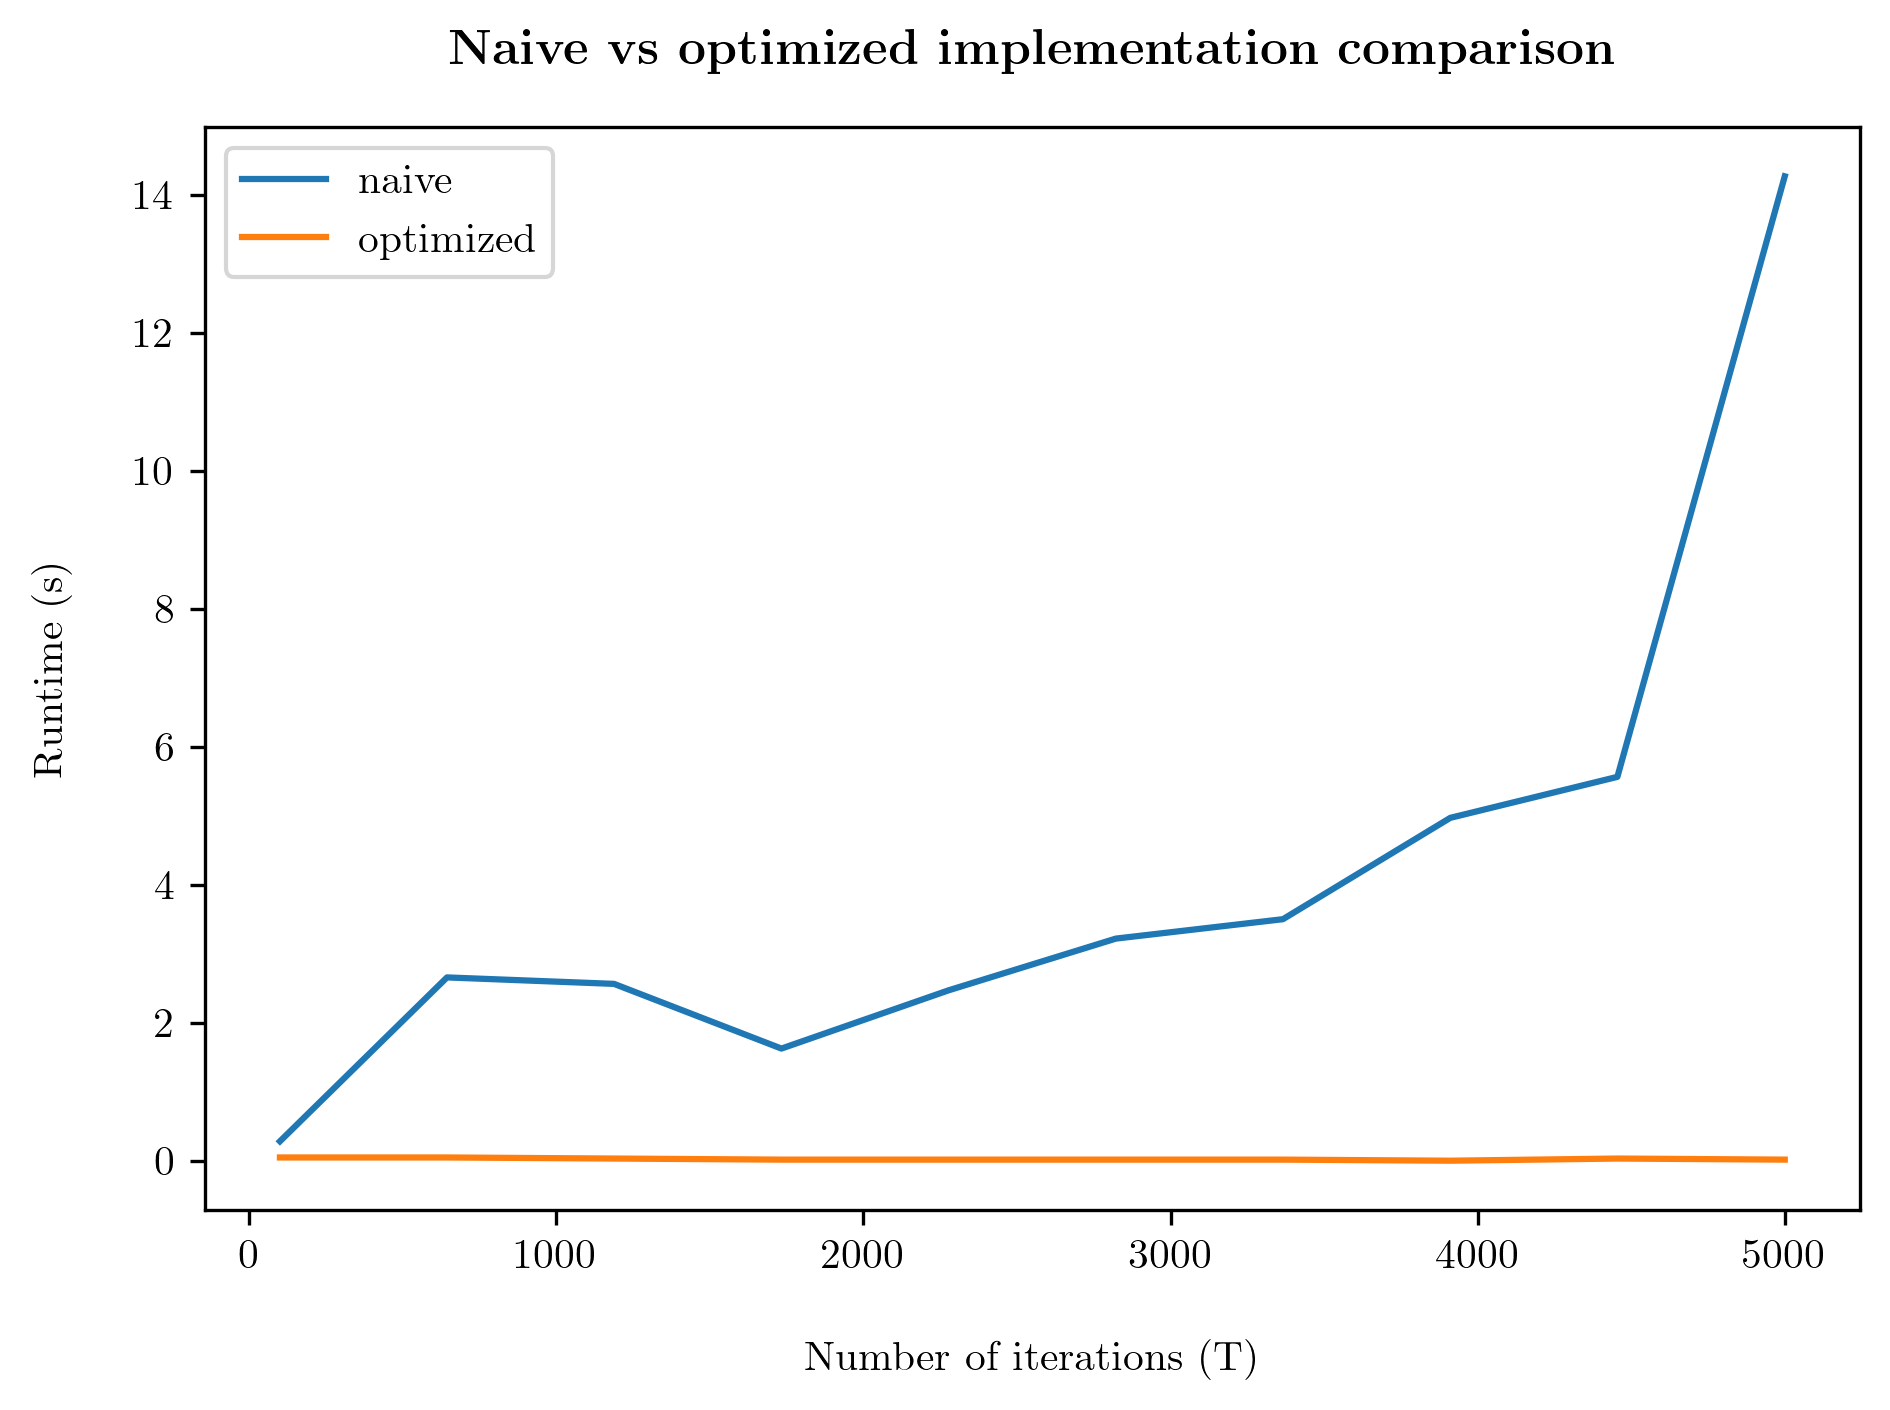
\includegraphics[width=0.8\textwidth]{../img/runtime.png}
  \caption{Runtime improvement when training a single binary classifier with the optimized Pegasos algorithm. The comparison was carried out using a custom training set with 1000 examples and a Gaussian kernel.} 
  \label{fig:algorithm:runtime}
\end{figure}

\section{Experiments}
\label{sec:experiments}

In this section we show the results of our experiments on the multiclass classification task using the Pegasos algorithm. The experiments were run on a machine with 16 gigabytes of RAM and a CPU Intel(R) Core(TM) i7-9700K 3.60GHz with 8 cores.

\subsubsection{Cross-validation.} The algorithm performance was evaluated with a 5-fold cross-validation on the entire USPS dataset. The folds were stratified so as to retain the proportion of the classes found in the complete dataset.

\subsubsection{Hyperparameters.} We investigated the behavior of the algorithm for different choices of the hyperparameters $T$ and $\lambda$, respectively representing the number of iterations and the regularization coefficient.

Concerning $T$, we gauged the performance of the algorithm over an increasing number of iterations, starting from a number much smaller than the cardinality of the training set and ending with a number several times bigger than the cardinality of the training set. More precisely, we chose the following values: 1000, 5000, 10000, 25000, 50000.

Concerning $\lambda$, in~\cite{shalev-pegasos-2011} the Pegasos algorithm was evaluated on the USPS dataset using $\lambda$ equal to $1.36 \times 10^{-4}$. It was also observed therein how, given a fixed number of iterations, the performance of the algorithm was inversely proportional to the value of $\lambda$, where $\lambda$ ranged from 1e-7 to 1e-3. The authors remarked that this behavior of the Pegasos algorithm for low values of $\lambda$ was known and attempts were being made to improve the performance for these values of the hyperparameter. We followed this insight, avoiding very low values of $\lambda$, and took the analysis one step further, experimenting with even higher values of $\lambda$, ranging from 1e-5 to 10.

We ran the algorithm with the polynomial and Gaussian kernel. The polynomial kernel was experimented upon with $n$ equal to 2, 3, 4 and 7, in order to assess the effectiveness of the algorithm at both low and high degrees of the polynomial. The Gaussian kernel was run with $\gamma$ equal to 0.25, as suggested in the project requirements, and also with $\gamma$ equal to 0.75 and 2. We note that in~\cite{shalev-pegasos-2011} the authors used $\gamma$ equal to $2$ on the USPS dataset.

\subsubsection{Results.} The cross-validated test error (zero-one loss) of the Pegasos algorithm over the USPS dataset with respect to the different training settings is shown in Figures~\ref{fig:experiments:polynomial_2}, \ref{fig:experiments:polynomial_3}, \ref{fig:experiments:polynomial_4}, \ref{fig:experiments:polynomial_7}, \ref{fig:experiments:gaussian_25}, \ref{fig:experiments:gaussian_75}, and \ref{fig:experiments:gaussian_2}.

Considering the training settings employing a polynomial kernel (Figures~\ref{fig:experiments:polynomial_2}, \ref{fig:experiments:polynomial_3}, \ref{fig:experiments:polynomial_4}, and \ref{fig:experiments:polynomial_7}), the best result is obtained using a degree of 3 (0.026), with degree 4 being very close (0.027). We can also observe how $\lambda$ plays a marginal role in determining the test error, with the exception of the test error measured when the degree is equal to 2. When using a degree of 7, the algorithm becomes completely insensitive to hyperparameter $\lambda$. Moreover, using a degree of 7 yields results that are generally worse across all choices of $T$, even when compared with degree 2. This is the telltale sign of overfitting.

Considering the training settings employing a Gaussian kernel (Figures~\ref{fig:experiments:gaussian_25}, \ref{fig:experiments:gaussian_75}, and \ref{fig:experiments:gaussian_2}), the best result is obtained with $\gamma$ equal to 2 (0.027). The hyperparameter $\lambda$ scarcely affects the performance of the algorithm when $\gamma$ is equal to 0.25 or 0.75, whereas it has a major effect when $\gamma$ is equal to 2. This behavior mirrors the one observed for the polynomial kernel, where overfitting hampered the effect of hyperparameter $\lambda$ and prevented the algorithm from reaching the best test error of lower degree polynomial kernels. On a related note, we remind that, for the Gaussian kernel, overfitting occurs when $\gamma$ is small with respect to the Euclidean distance between two examples. Contrary to what was observed in~\cite{shalev-pegasos-2011}, the algorithm yields a better test error when using low values of $\lambda$, at least within the investigated interval. This can be noticed across all values of $\gamma$ and all values of $T$.

Surprisingly, the overall best setting for the polynomial kernel outperforms the overall best setting for the Gaussian kernel, albeit by a small margin. However, the best setting for the Gaussian kernel is consistently better than the best setting for the polynomial kernel when using a small number of iterations (namely, 1000, 5000, 10000, 25000). In addition, the overall best setting for the Gaussian kernel reaches its lowest test error faster than the overall best setting for the polynomial kernel. Indeed, while the polynomial kernel with degree 3 reaches 0.026 test error with 50000 iterations, the Gaussian kernel with $\gamma$ equal to 2 reaches 0.027 test error with half the iterations.

Finally, Figure~\ref{fig:experiments:cv_runtime} shows the runtime of the algorithm for the different values of $T$, averaged with respect to the values of $\lambda$. From this figure we infer that training with the Gaussian kernel requires significantly more time than training with the polynomial kernel across all the values of $T$. The runtime presents also an upward trend when increasing the number of iterations, although the growth is slow and seemingly linear in the number of iterations. 

\begin{figure}
  \center
  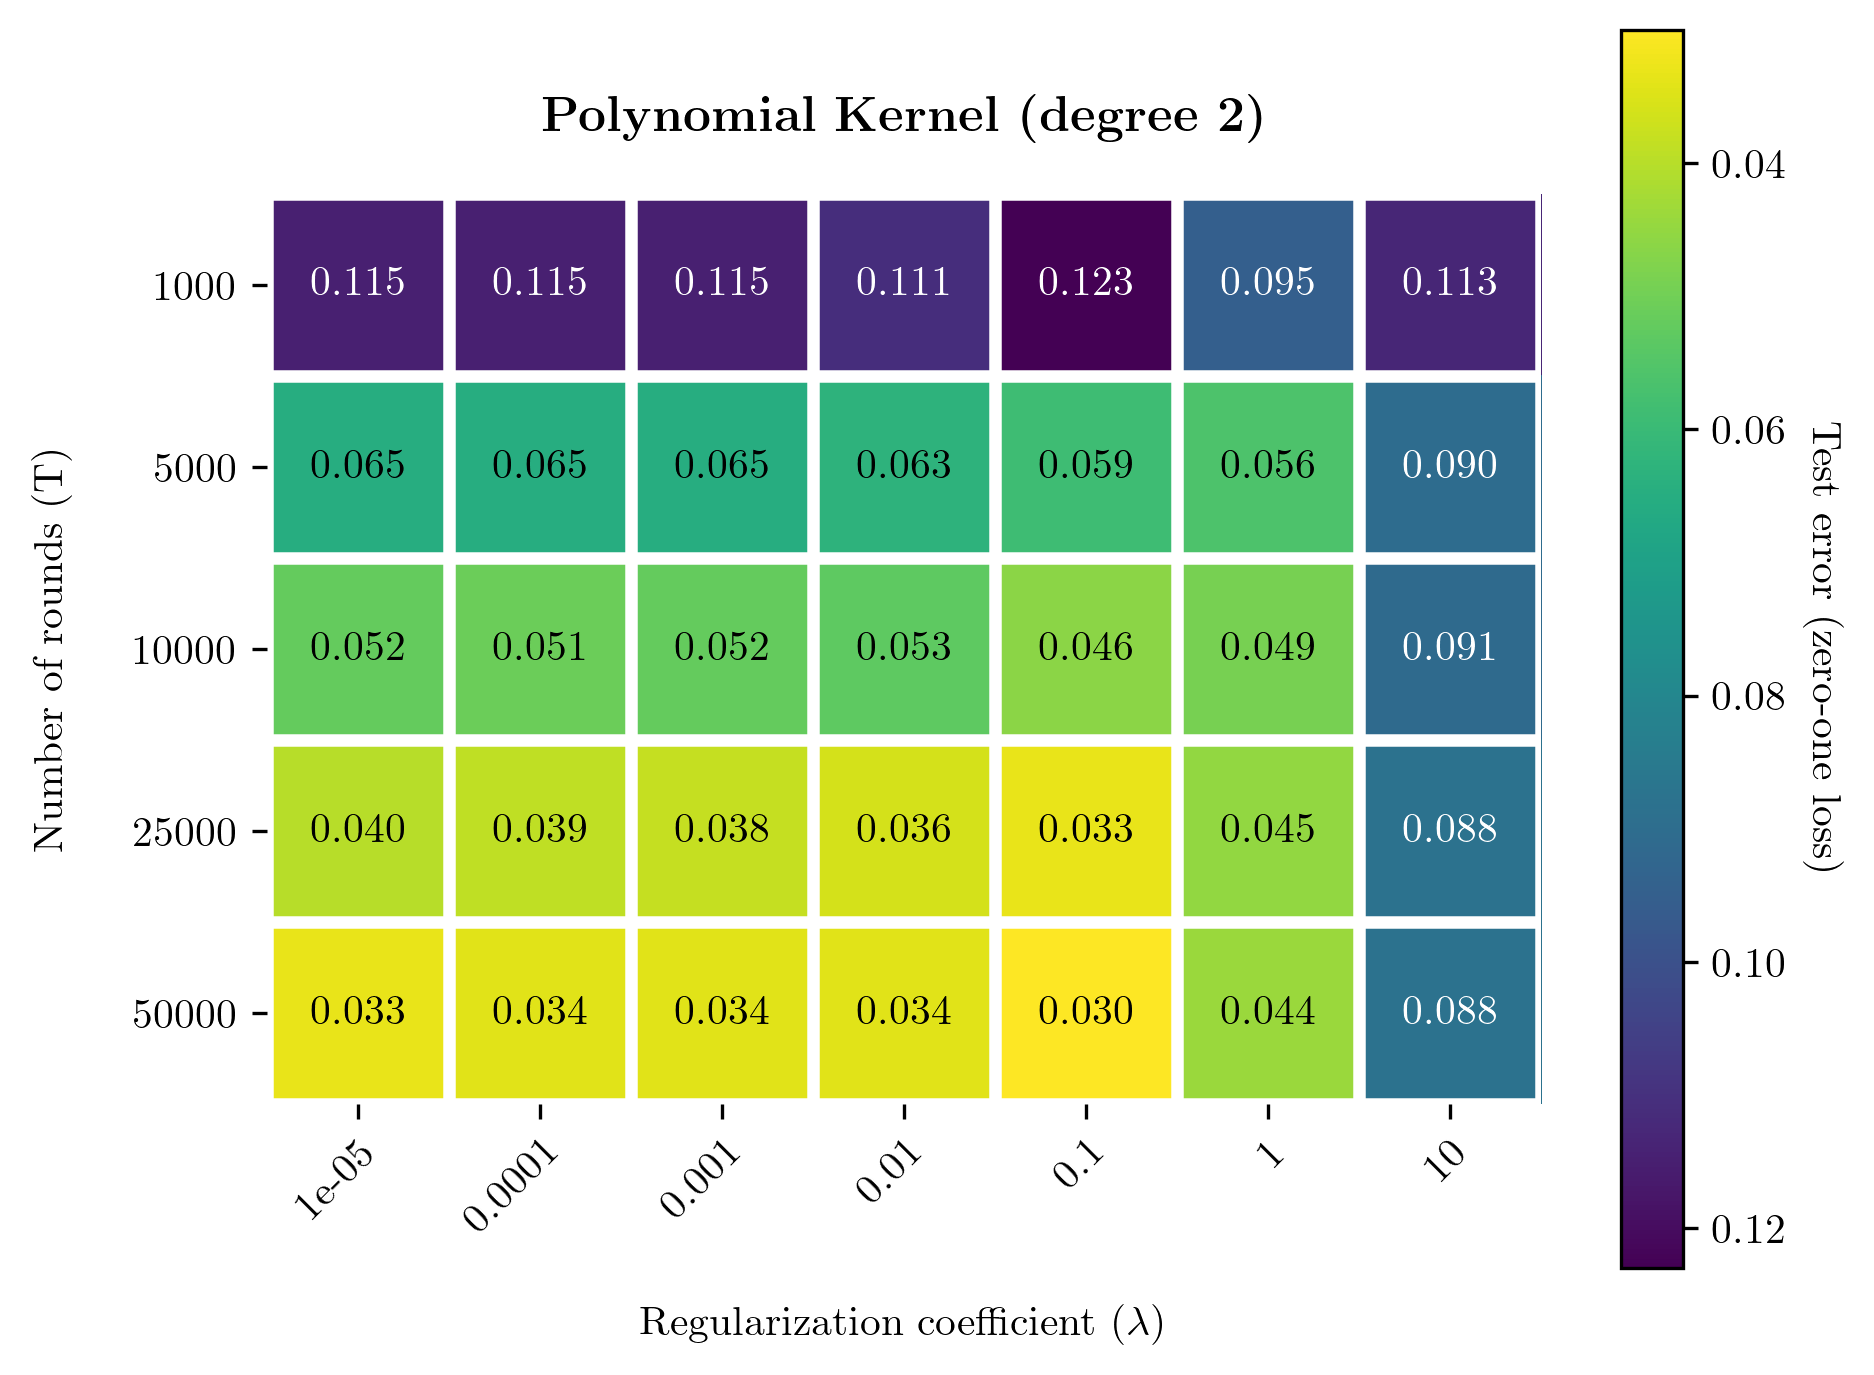
\includegraphics[width=0.8\linewidth]{../img/poly_2_error.png}
  \caption{5-fold cross-validated test error (zero-one loss) of the Pegasos algorithm for multiclass classification over the USPS dataset, employing a polynomial kernel of degree 2.} 
  \label{fig:experiments:polynomial_2}
\end{figure}

\begin{figure}
  \center
  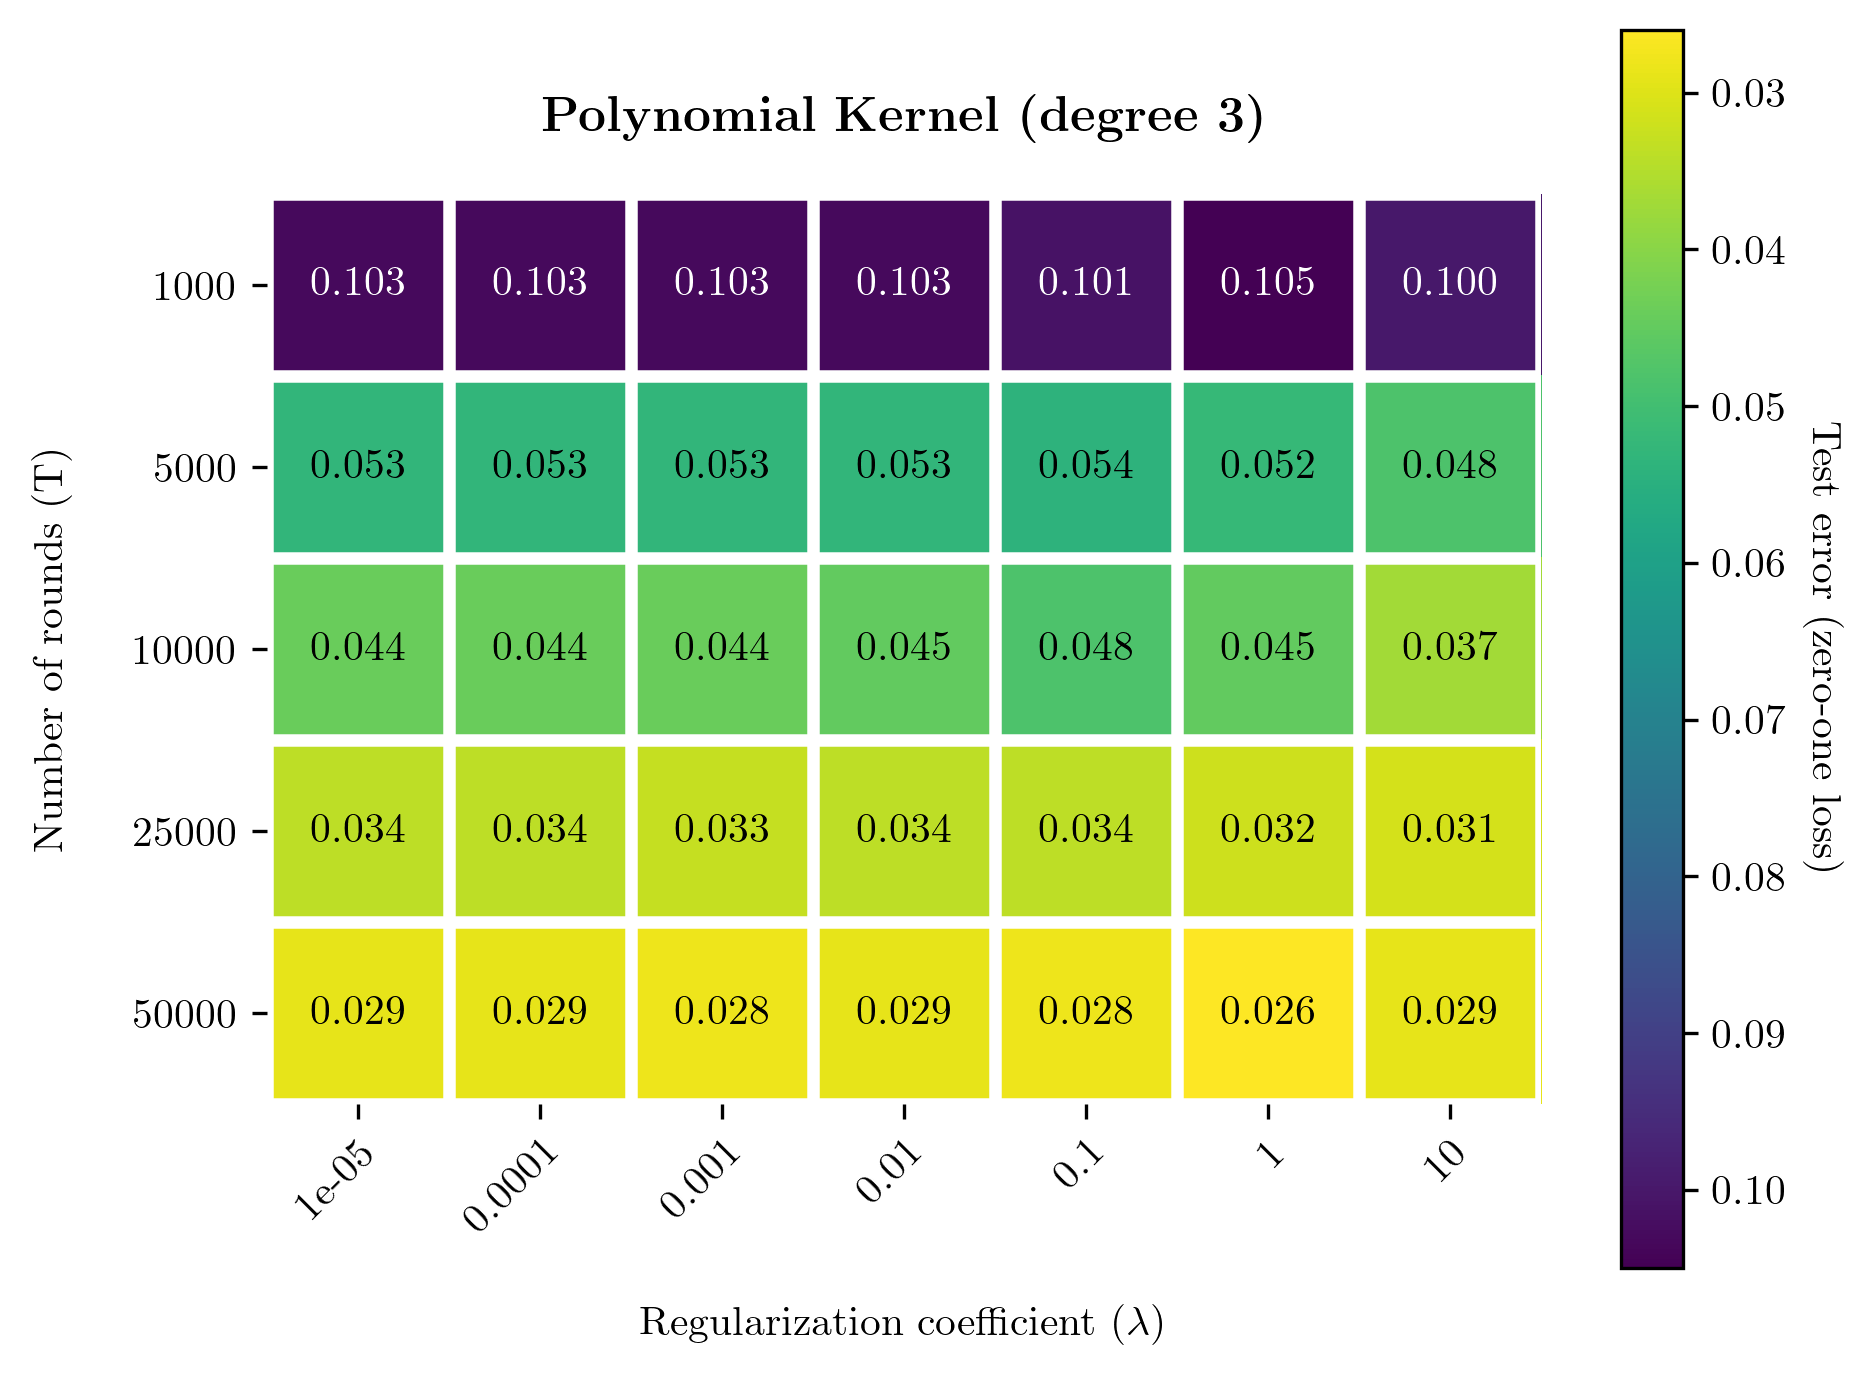
\includegraphics[width=0.8\linewidth]{../img/poly_3_error.png}
  \caption{5-fold cross-validated test error (zero-one loss) of the Pegasos algorithm for multiclass classification over the USPS dataset, employing a polynomial kernel of degree 3.} 
  \label{fig:experiments:polynomial_3}
\end{figure}

\begin{figure}
  \center
  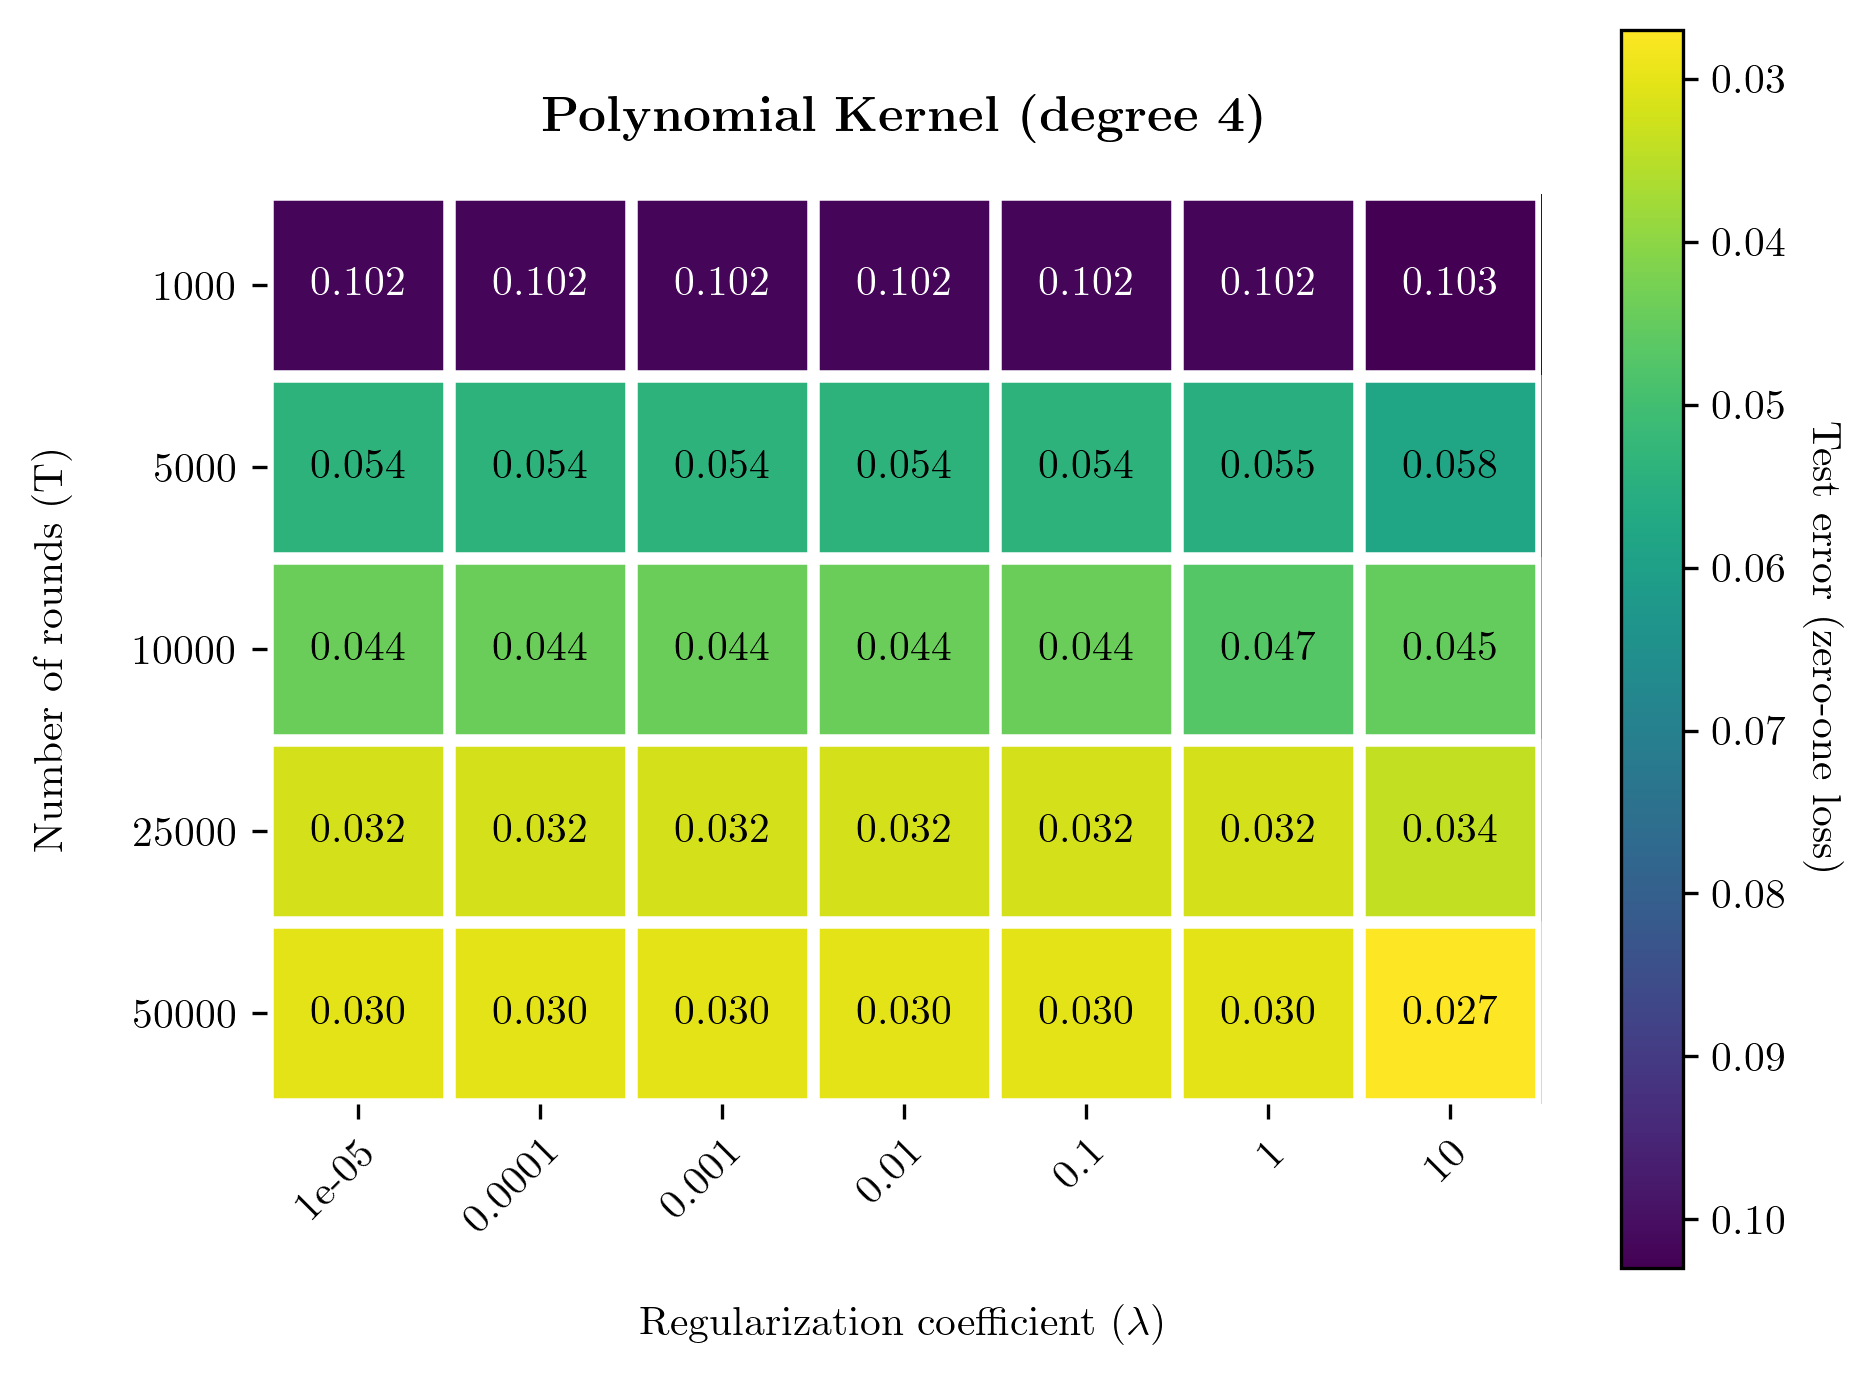
\includegraphics[width=0.8\linewidth]{../img/poly_4_error.png}
  \caption{5-fold cross-validated test error (zero-one loss) of the Pegasos algorithm for multiclass classification over the USPS dataset, employing a polynomial kernel of degree 4.} 
  \label{fig:experiments:polynomial_4}
\end{figure}

\begin{figure}
  \center
  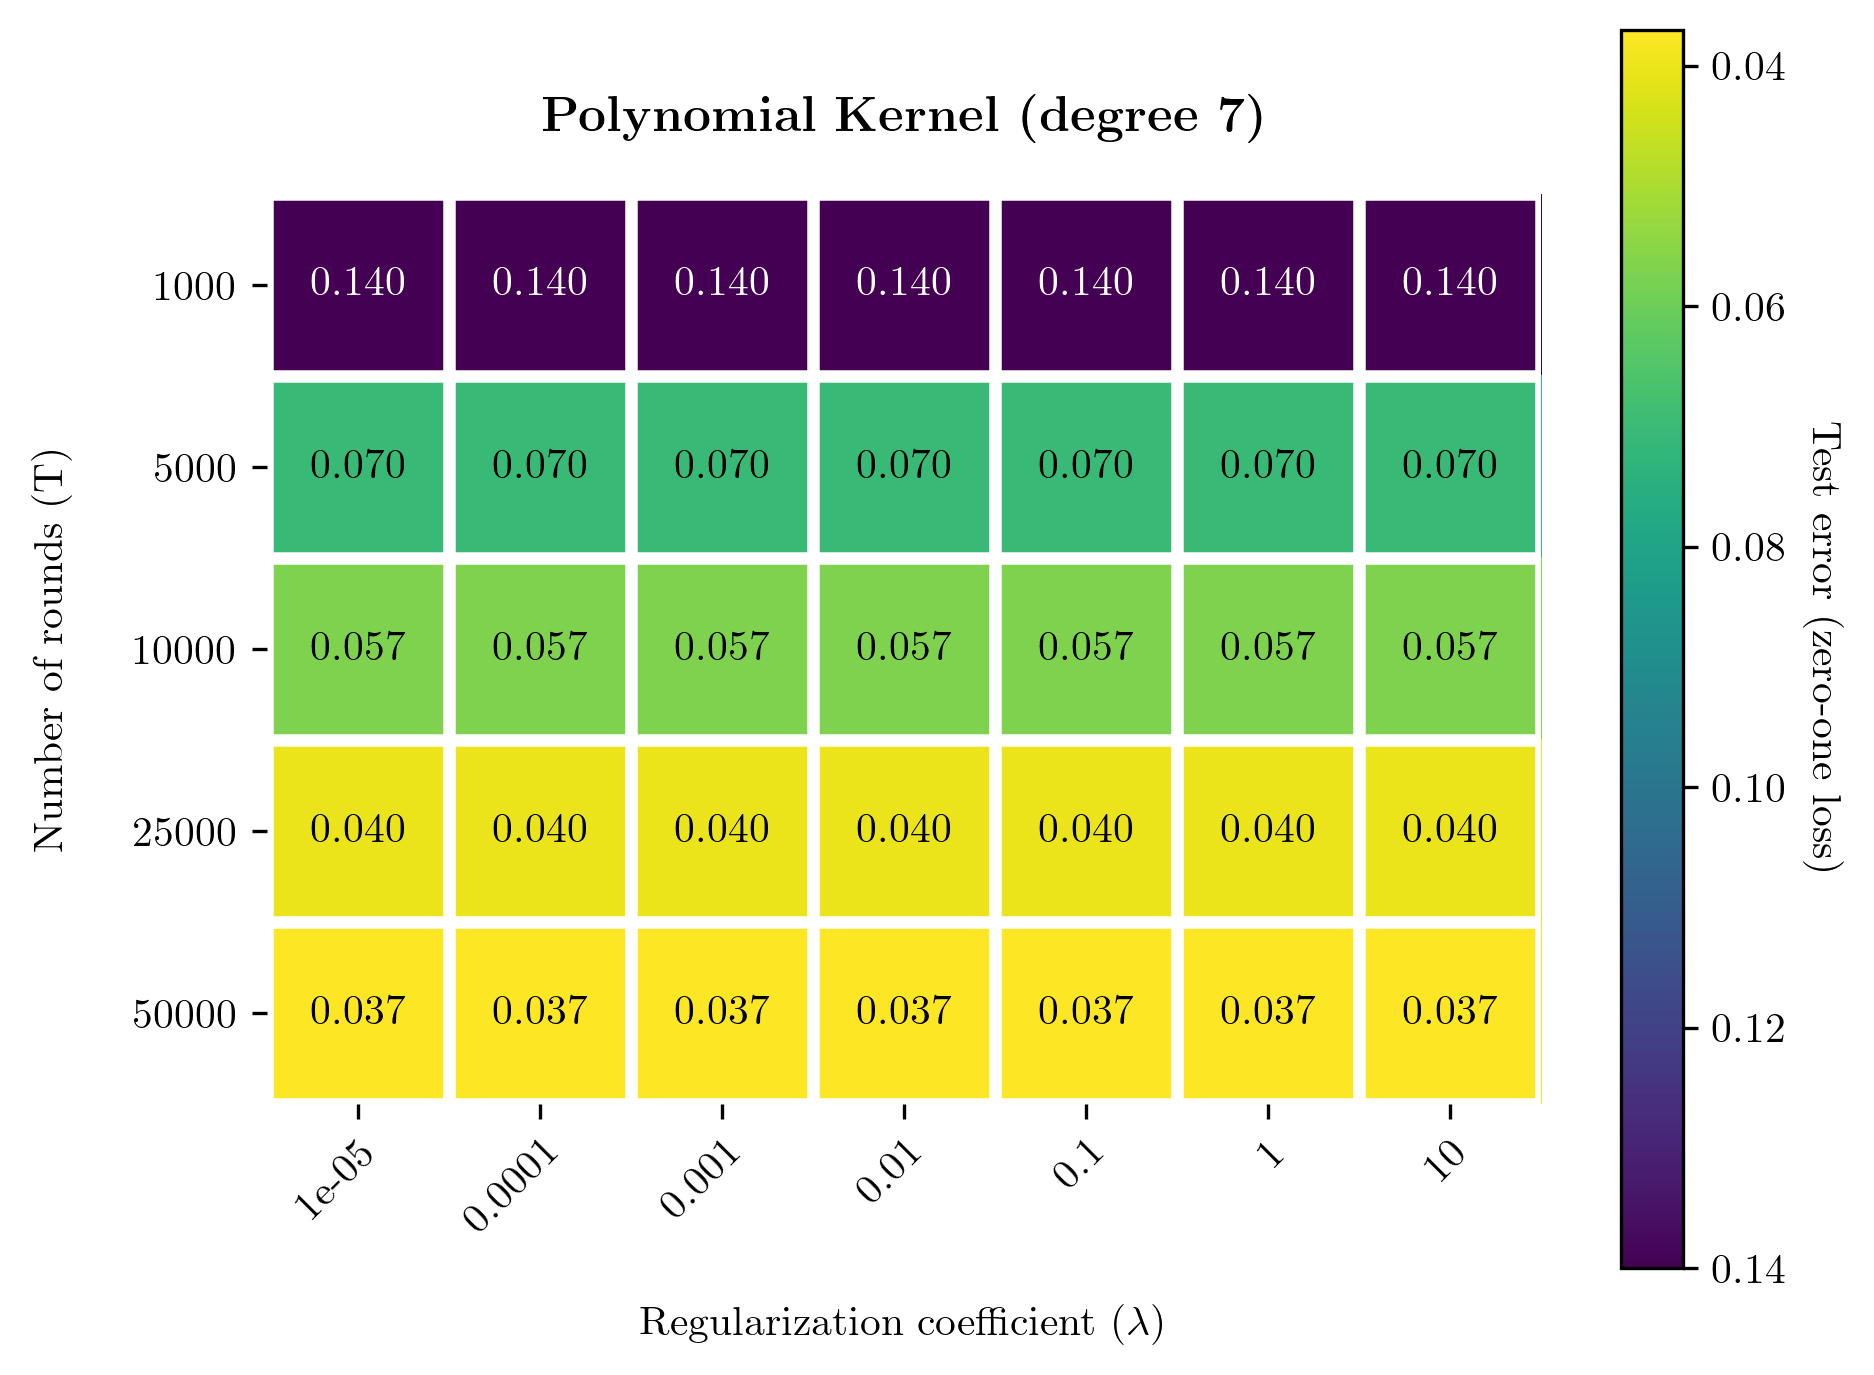
\includegraphics[width=0.8\linewidth]{../img/poly_7_error.png}
  \caption{5-fold cross-validated test error (zero-one loss) of the Pegasos algorithm for multiclass classification over the USPS dataset, employing a polynomial kernel of degree 7.} 
  \label{fig:experiments:polynomial_7}
\end{figure}

\begin{figure}
  \center
  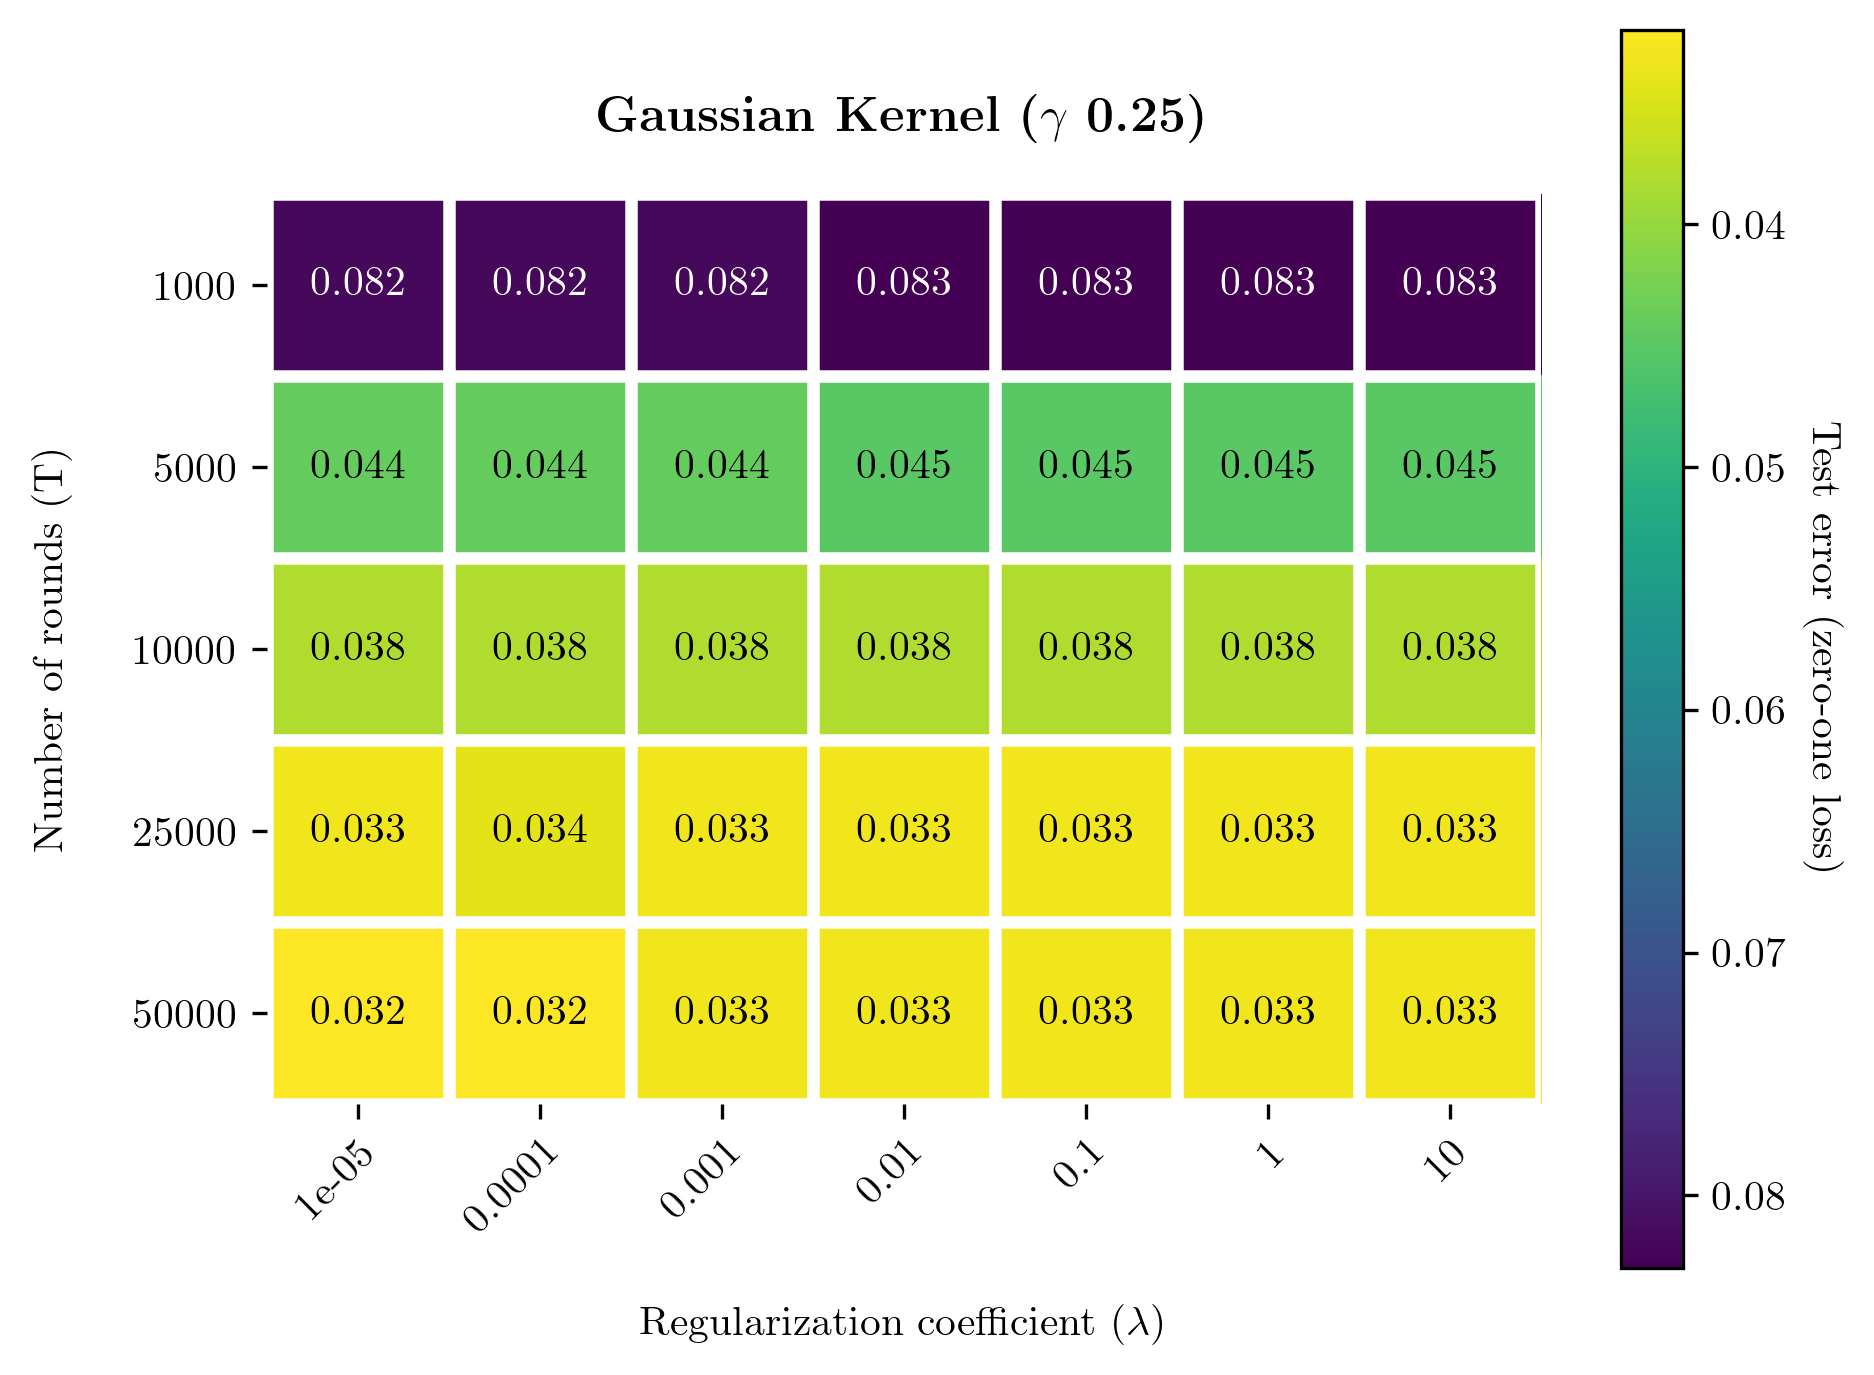
\includegraphics[width=0.8\linewidth]{../img/gaussian_25_error.png}
  \caption{5-fold cross-validated test error (zero-one loss) of the Pegasos algorithm for multiclass classification over the USPS dataset, employing a Gaussian kernel with $\gamma$ equal to 0.25.} 
  \label{fig:experiments:gaussian_25}
\end{figure}

\begin{figure}
  \center
  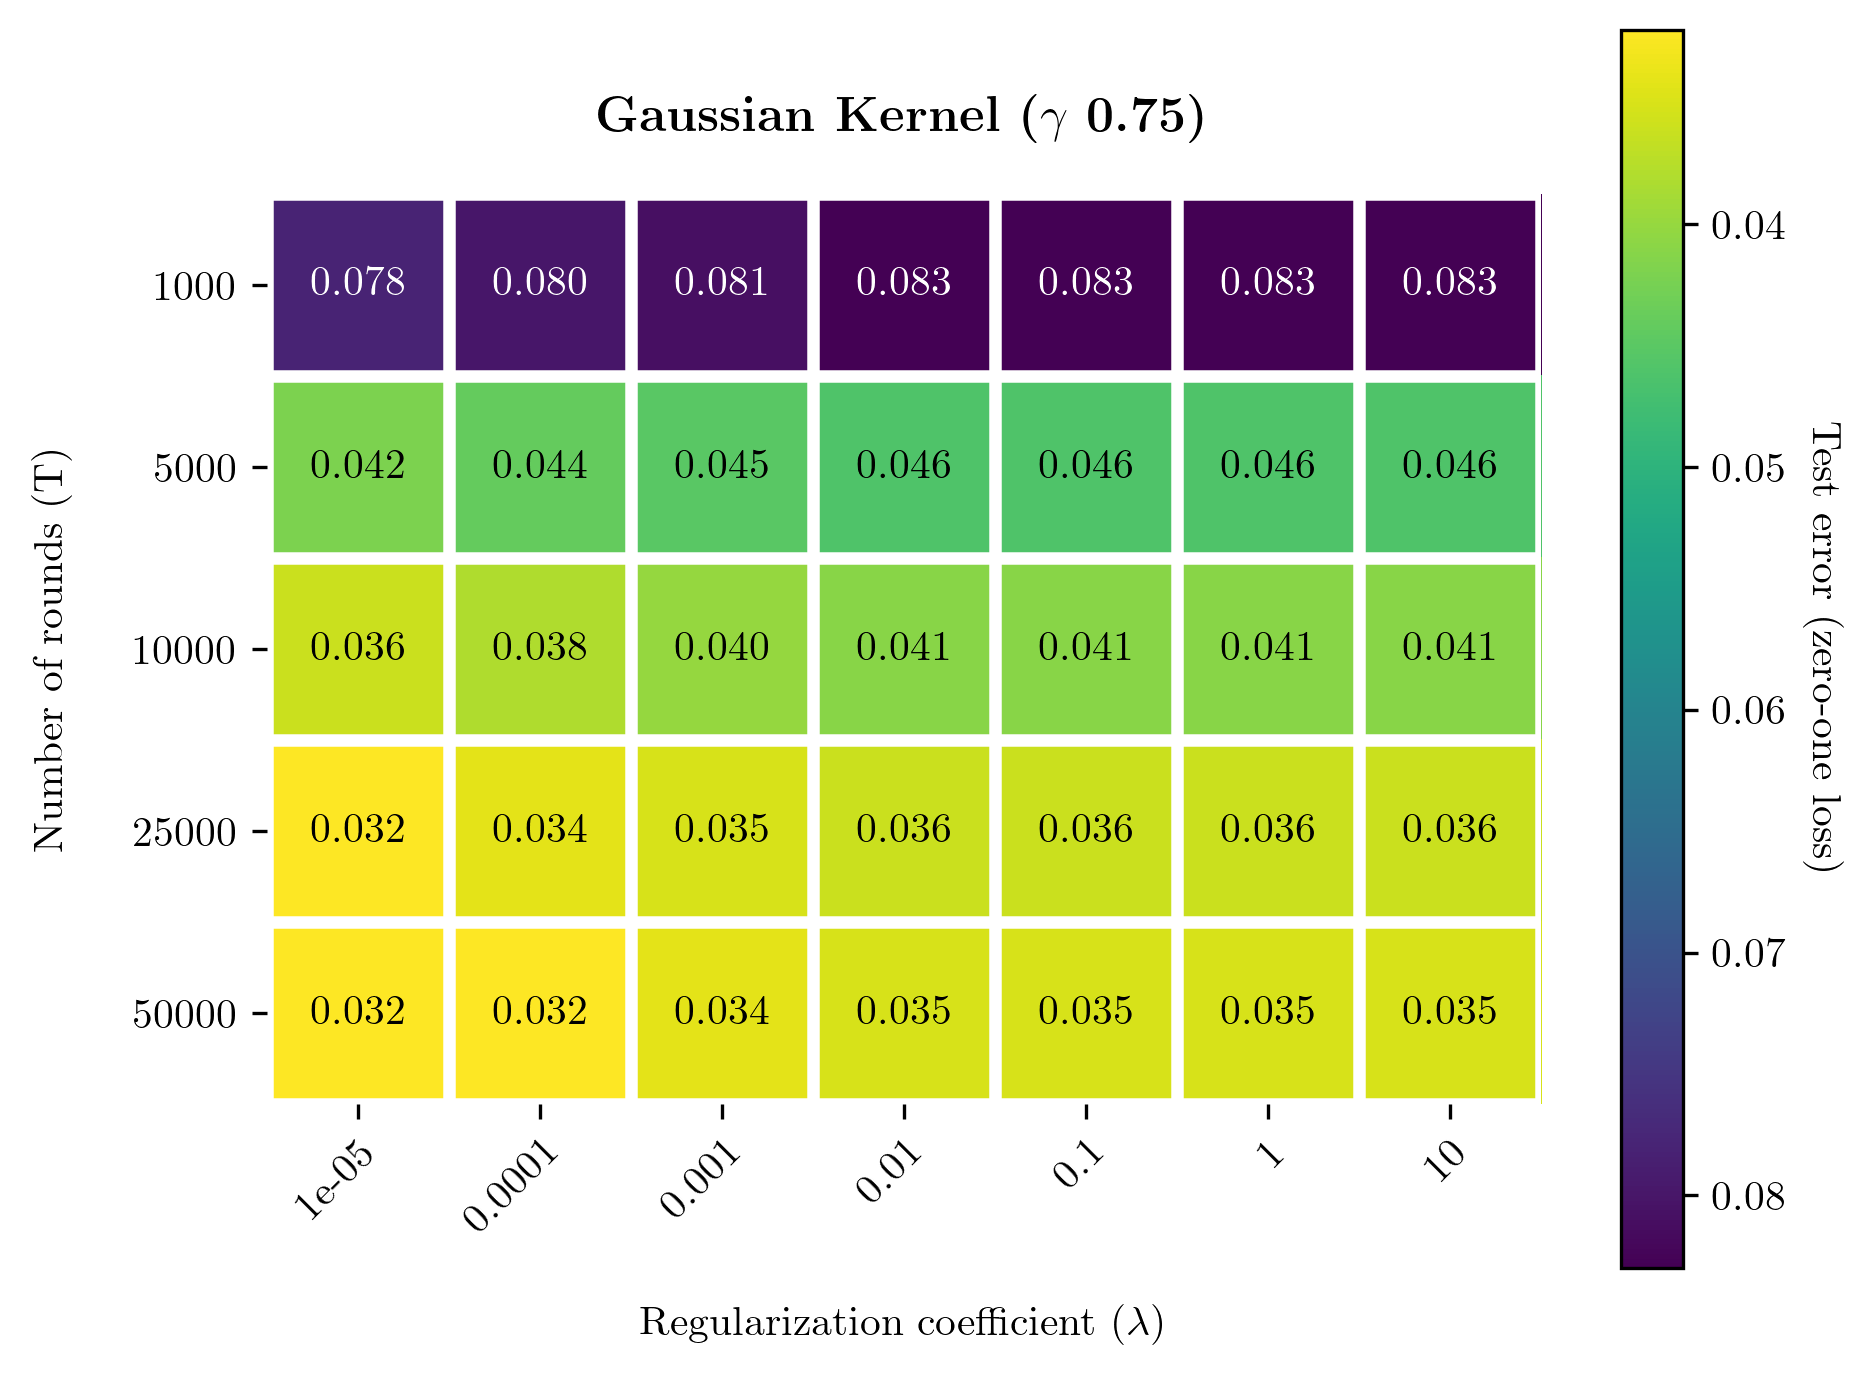
\includegraphics[width=0.8\linewidth]{../img/gaussian_75_error.png}
  \caption{5-fold cross-validated test error (zero-one loss) of the Pegasos algorithm for multiclass classification over the USPS dataset, employing a Gaussian kernel with $\gamma$ equal to 0.75.} 
  \label{fig:experiments:gaussian_75}
\end{figure}

\begin{figure}
  \center
  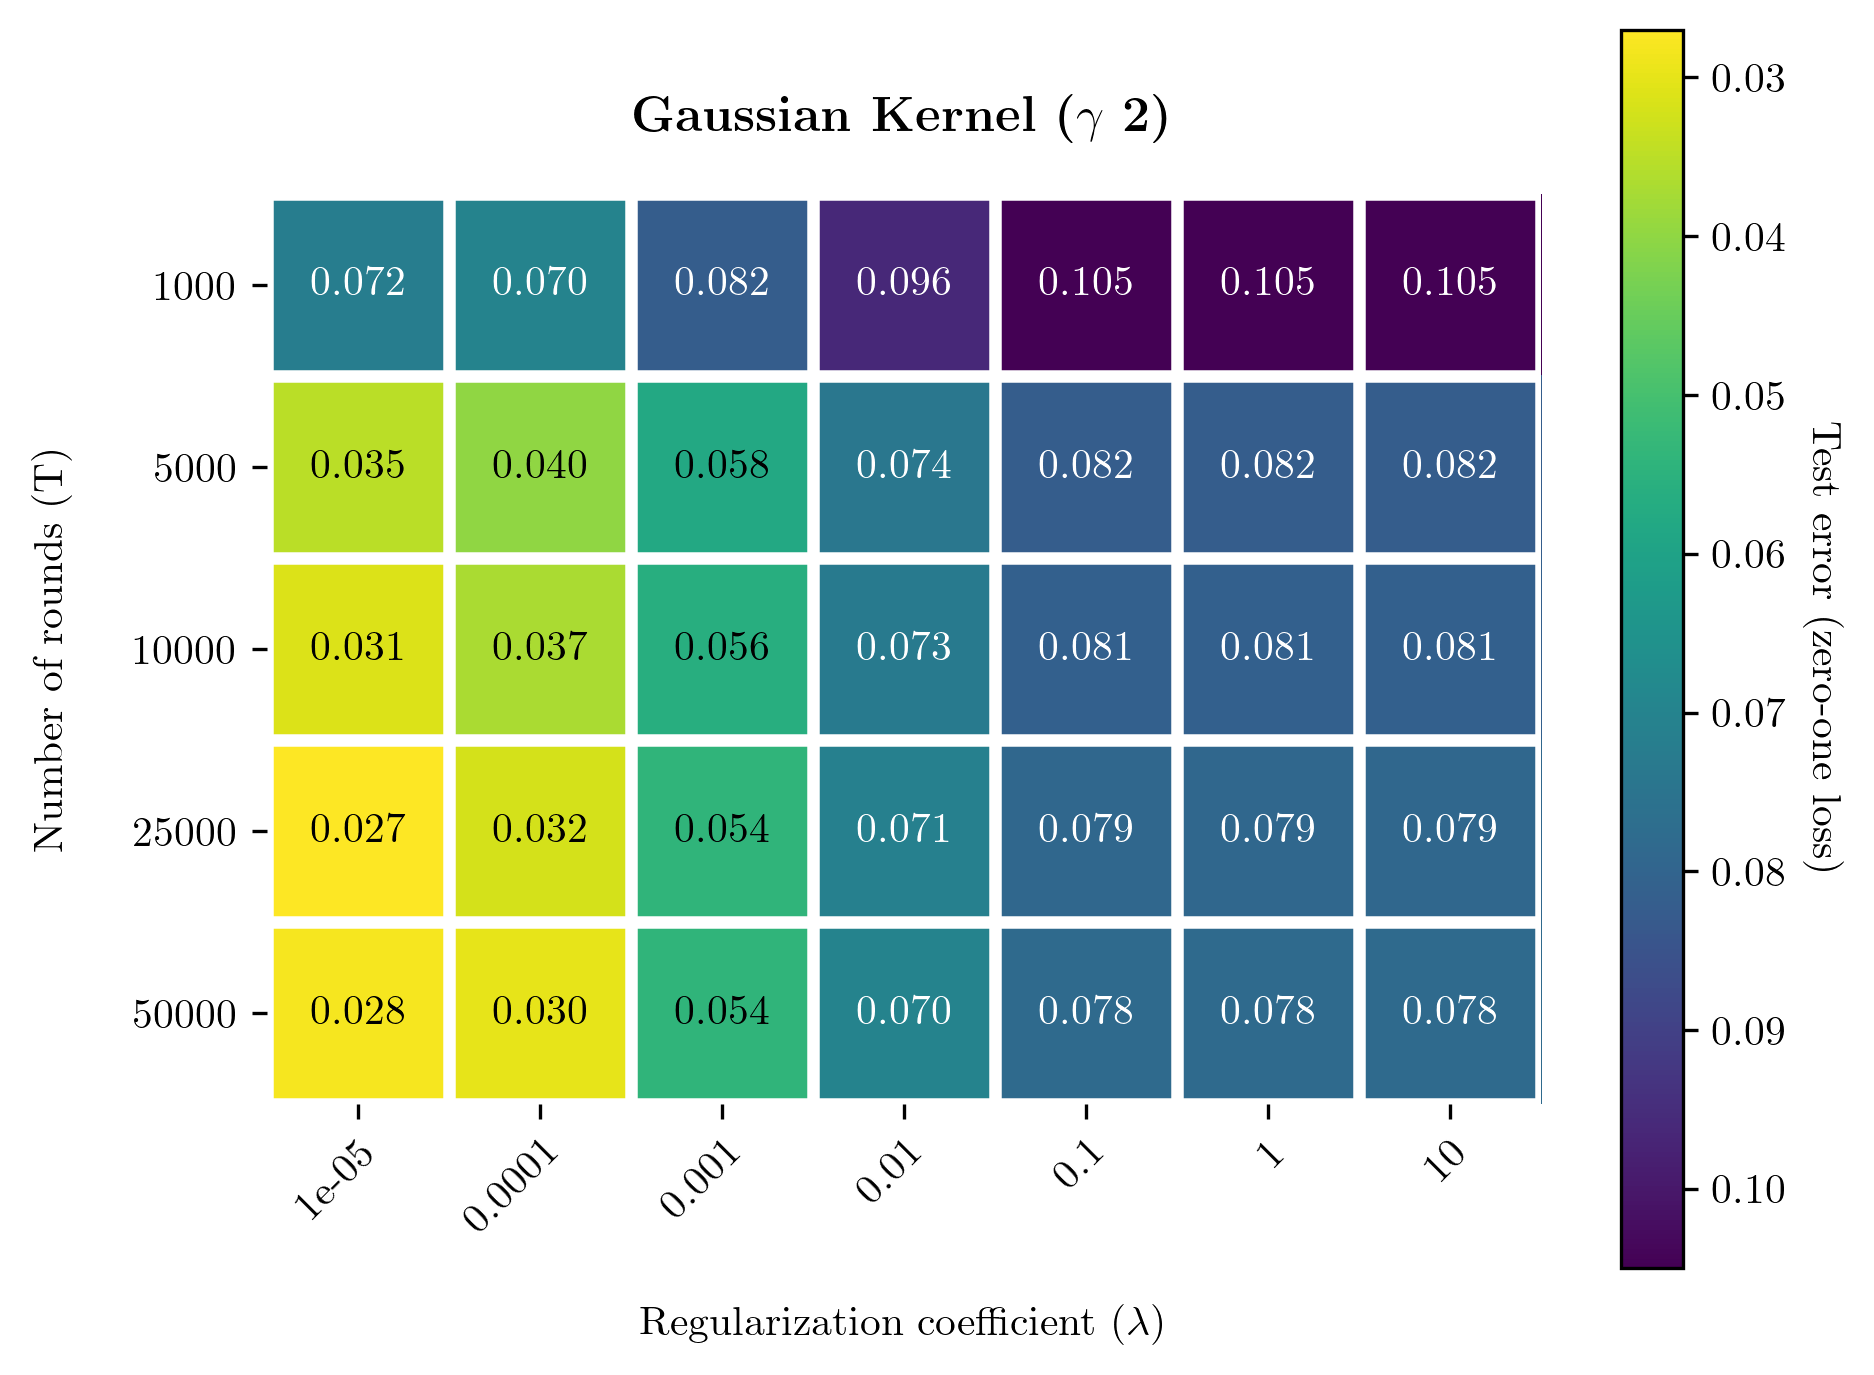
\includegraphics[width=0.8\linewidth]{../img/gaussian_2_error.png}
  \caption{5-fold cross-validated test error (zero-one loss) of the Pegasos algorithm for multiclass classification over the USPS dataset, employing a Gaussian kernel with $\gamma$ equal to 2.} 
  \label{fig:experiments:gaussian_2}
\end{figure}

\begin{figure}
  \center
  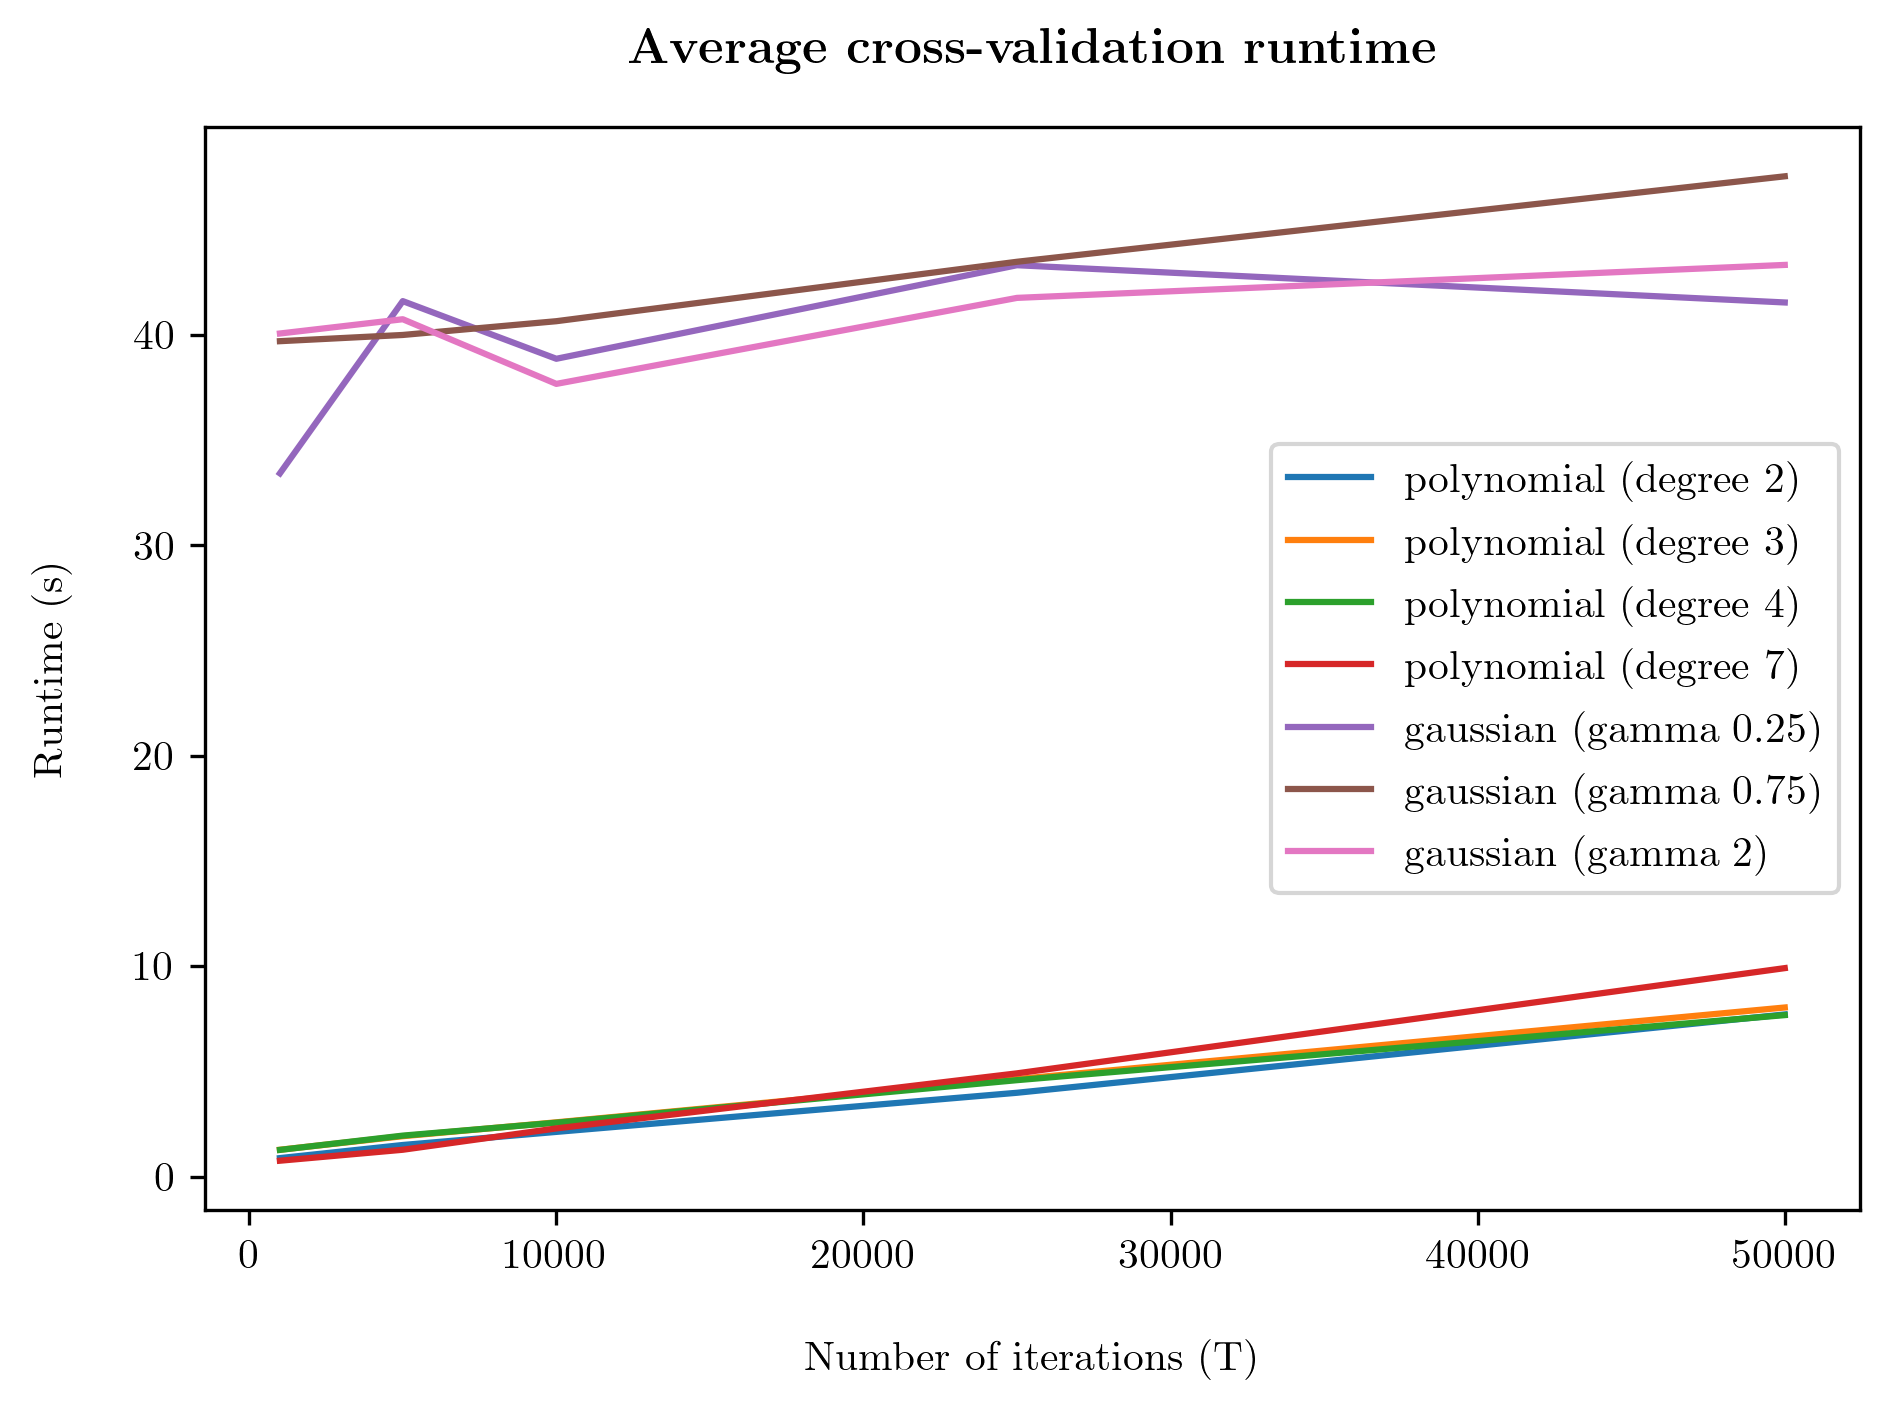
\includegraphics[width=0.8\linewidth]{../img/cv_runtime.png}
  \caption{Runtime of the Pegasos algorithm for multiclass classification over the USPS dataset across the different values of $T$, averaged with respect to the values of $\lambda$.} 
  \label{fig:experiments:cv_runtime}
\end{figure}

\section{Conclusions}
\label{sec:conclusions}

In this work we investigated the performance of the Pegasos algorithm described in Section~\ref{sec:algorithm} on a multiclass classification task over the USPS dataset described in Section~\ref{sec:dataset}. The algorithm was evaluated with 5-fold stratified cross-validation across various settings of hyperparameters. The best performance (0.026 test error with zero-one loss) was achieved by using a polynomial kernel of degree 3, 50000 iterations and a regularization coefficient of 1. A similar performance (0.027 test error) was achieved by using a Gaussian kernel with $\gamma$ equal to 2, 25000 iterations and a regularization coefficient of 1e-5.

The algorithm proved to be an effective classification tool, although the task was not particularly challenging. Moreover, the algorithm showed a noteworthy rate of convergence, bordering a test error of 0.070 after only 1000 iterations when using the Gaussian kernel with $\gamma$ equal to 2.

Further research might explore a wider set of hyperparameters, especially in the direction of lower regularization coefficient values and higher values of $\gamma$ when using a Gaussian kernel.

\section*{Statement}
\textit{I/We declare that this material, which I/We now submit for assessment, is entirely my/our own work and has not been taken from the work of others, save and to the extent that such work has been cited and acknowledged within the text of my/our work. I/We understand that plagiarism, collusion, and copying are grave and serious offences in the university and accept the penalties that would be imposed should I engage in plagiarism, collusion or copying. This assignment, or any part of it, has not been previously submitted by me/us or any other person for assessment on this or any other course of study.}

\bibliographystyle{acm}
\bibliography{bibtex_entries}

\end{document}